\documentclass[10pt,twocolumn]{article}

\usepackage[a4paper,margin=18mm,columnsep=7mm]{geometry}
\usepackage{amsmath,amssymb,mathtools,booktabs,array,multirow}
\usepackage{graphicx}
\usepackage{microtype}
\usepackage{xcolor}
\usepackage{cite}
\usepackage{url}
\usepackage[hidelinks]{hyperref}
\hypersetup{
  pdftitle={Role-Anchored Update Authorisation: Defending Temporal Graph Intrusion Detection Against Slow Memory Drift},
  pdfauthor={Mohamed Amine EL KALAI}
}
\usepackage{pifont}
\newcommand{\cmark}{\ding{51}}
\newcommand{\xmark}{\ding{55}}
\usepackage{tikz}
\usetikzlibrary{arrows.meta,positioning,fit,shapes.geometric,calc,backgrounds,decorations.pathreplacing}
\usepackage{enumitem}
\usepackage{caption}
\usepackage{placeins}
\usepackage{float}
\usepackage{balance}
\usepackage{dblfloatfix}

\setlength{\parindent}{1em}
\setlength{\parskip}{0pt}
\setlength{\textfloatsep}{8pt plus 2pt minus 2pt}
\setlength{\floatsep}{6pt plus 2pt minus 2pt}
\setlength{\intextsep}{6pt plus 2pt minus 2pt}
\setlist{nosep,leftmargin=*}
\raggedbottom

\definecolor{tgnblue}{HTML}{2C6EAA}
\definecolor{attackred}{HTML}{B33A3A}
\definecolor{defgreen}{HTML}{3A7D44}
\definecolor{amber}{HTML}{B26A00}
\definecolor{purple}{HTML}{6B4C9A}
\definecolor{softgray}{HTML}{F2F4F7}

\tikzset{
  block/.style={draw,rounded corners=2pt,align=center,minimum height=7mm,
    fill=softgray,font=\scriptsize,inner sep=3pt},
  attack/.style={block,draw=attackred,fill=attackred!8},
  defend/.style={block,draw=defgreen,fill=defgreen!8},
  data/.style={block,draw=tgnblue,fill=tgnblue!7},
  proposed/.style={block,draw=purple,fill=purple!7},
  flow/.style={-{Latex[length=2mm]},thick}
}

\title{\vspace{-1em}\textbf{Role-Anchored Update Authorisation:\\[2pt]
Defending Temporal Graph Intrusion Detection\\[2pt]
Against Slow Memory Drift}\vspace{-0.6em}}
\author{Mohamed Amine EL KALAI}
\date{}

\begin{document}
\maketitle
\vspace{-1.5em}

% =====================================================================
\begin{abstract}
Temporal Graph Networks (TGNs) underpin state-of-the-art provenance-based
intrusion detection systems such as KAIROS by maintaining per-node recurrent
memory that conditions anomaly scoring.  We identify an unexplored attack
surface in this memory mechanism: an adversary controlling a compromised
identity issues sub-threshold interactions that gradually steer node memory,
thereby suppressing the anomaly score of a subsequent malicious payload.  We
term this a \emph{slow memory drift} attack and demonstrate that the
conditioning phase evades plain KAIROS at every tested injection rate
(1--100 events/hour, 91.7--99.8\% event-level stealth).

We propose \emph{Role-Anchored Update Authorisation}, a complementary defence
layer that monitors five drift signals (role displacement, update innovation,
directional persistence, trajectory coherence, and event surprise) through a
gap-reset CUSUM sequential monitor.  The defence requires \textbf{zero
trainable neural parameters}; it operates solely on the frozen KAIROS
checkpoint and clean-validation statistics.  Signal weights are optimised
to emphasise \emph{movement-pattern} signals (persistence and coherence)
over \emph{position} signals (displacement and surprise), which increases
rate coverage from 1/12 to 7/12 on the evaluated scenario.

Evaluated on (i)~the frozen DARPA CADETS~E3 checkpoint~\cite{darpa2018tc}
in a four-branch difference-in-differences~\cite{angrist2009mostly} design
across \textbf{12~injection rates} (1--100~events/hour) and (ii)~the
CMU CERT~r4.2 insider-threat corpus~\cite{lindauer2020cert} with
\textbf{70~labelled insiders} across 3~attack scenarios, 5~independently
trained TGN checkpoints, and a \textbf{10-month longitudinal} event stream
of 15.6~million events, the defence:
\begin{itemize}[nosep]
  \item detects conditioning at \textbf{7/12} rates with
    \textbf{zero false positives} on the CADETS checkpoint (early warning
    1.1--9.9~h, causal payoff recovery $R{=}+0.135$,
    CI~$[+0.113,\;+0.160]$);
  \item on CERT~r4.2, the combined KAIROS\,+\,defence system detects
    \textbf{10/10} Scenario~3 insiders (vs.\ 9/10 for plain KAIROS),
    \textbf{28/30} Scenario~2 insiders (vs.\ 26/30), and
    \textbf{26/30} Scenario~1 insiders (vs.\ 23/30), based on
    majority-vote across 5~seeds;
  \item achieves a positive net detection rate ($+0.114$ on the best seed)
    across the full 70-insider corpus while maintaining the base detector's
    recall on all three attack scenarios.
\end{itemize}
A non-monotonic detection boundary emerges on CADETS: the defence detects
rate~4 but not rates~6 or~8, stabilising to full detection at rate~10 and
above.  The multi-target CERT evaluation confirms that role-anchored
monitoring generalises across attack types, temporal positions, and
independently trained checkpoints, providing evidence that it serves as a
practical, zero-cost complement to TGN-based intrusion detection.
Code and data are available at
\url{https://github.com/SpaceAttay3154518/TGN-UEBA}.
\end{abstract}

% =====================================================================
\section{Related Work}
\label{sec:related}

\subsection{Graph-based intrusion detection}

Graphs encode the contextual relationships that distinguish benign system
events from malicious ones.  A recent survey organises graph neural network
(GNN) approaches to intrusion detection along the axes of graph construction,
relational feature learning, and operational deployment~\cite{zhong2024gidssurvey}.
Flow-based designs such as E-GraphSAGE~\cite{lo2022egraphsage} and
Anomal-E~\cite{caville2022anomale} apply neighbourhood aggregation to
network-flow graphs; however, a fixed flow table differs fundamentally from
a causal, continuously updating provenance graph.

Whole-system provenance IDSs~\cite{king2003backtracking,bates2015trustworthy}
represent kernel objects (processes, files,
sockets) as typed nodes and information-flow events as directed, timestamped
edges.  KAIROS~\cite{cheng2024kairos}, the primary reference system in this
work, is a TGN-derived encoder-decoder that scores streaming provenance
events and correlates anomalous 15-minute windows into compact attack
summary graphs.  FLASH~\cite{rehman2024flash} combines semantic attributes
with provenance representation learning; TAPAS~\cite{zhang2025tapas} reduces
redundancy via process-centric segmentation; and
ORTHRUS~\cite{jiang2025orthrus} shifts focus toward \emph{attribution
quality}, reducing the subgraph an analyst must inspect.  Recent architectures
such as Trace2Vec~\cite{liu2025trace2vec},
DYNAMO~\cite{wang2026dynamo}, and TKnet~\cite{wang2026tknet} explore richer
temporal encoders but remain focused on representation accuracy rather than
the integrity of the recurrent state that produces those representations.

A recent unified evaluation of eight provenance
IDSs~\cite{bilot2025simpler} reinforces the need for careful benchmarking:
simple models can remain competitive under controlled metrics, and
substantial discrepancies arise from dataset scale and preprocessing
choices.

\subsection{Adversarial attacks on temporal GNNs}

The threat landscape for temporal GNNs spans training-time poisoning and
test-time evasion.  T-SPEAR~\cite{lee2024spear} poisons continuous-time
training data with temporally plausible edges; HIA~\cite{jeon2025hia} selects
influential nodes before adding or deleting edges;
LoReTTA~\cite{pal2025loretta} removes influential edges and inserts
distribution-preserving adversarial negatives.  Provenance
mimicry~\cite{goyal2023mimicry} adds benign-looking activity around malicious
processes at test time.  All of these operate on the graph \emph{structure}
rather than exploiting the recurrent memory mechanism.

MemFreezing~\cite{dai2025memfreezing} is the closest prior work: it
explicitly attacks TGN memory by injecting crafted fake messages to freeze
node states.  However, its objective is persistent
\emph{generic degradation}, not payoff-directed normalisation.  The slow
memory drift attack we formalise differs in three fundamental ways: it
operates through \emph{observed} events (not synthetic messages), unfolds
over \emph{many timestamps} (not a single injection), and targets the
\emph{suppression of a specific payoff score} (not indiscriminate disruption).

We verify this distinction empirically using a MemFreezing discrimination
test on an adapted TGN (CERT~r4.2~\cite{lindauer2020cert}, 3~seeds, 57~attack events,
237~root-benign events, 15,441~other-benign events).
Figure~\ref{fig:memfreeze} summarises the results.  MemFreezing
\emph{increases} attack-event anomaly scores by $+0.143$ on average
(95\%~CI $[+0.070,\;+0.224]$), making victims \emph{more} conspicuous,
the opposite of slow drift's $-0.004$ suppression.  The alert rate for
attack events rises from 7.0\% to 15.8\% under MemFreezing, further
confirming that the two attacks have opposite effects on detectability.

\begin{figure}[htbp]
\centering
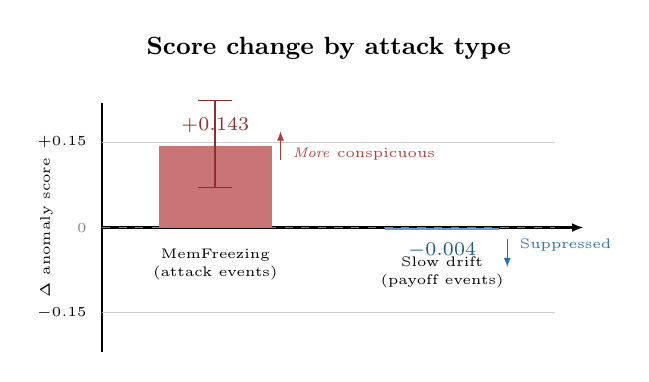
\begin{tikzpicture}[scale=0.72]
  % Title
  \node[font=\small\bfseries,anchor=south] at (4,5.3) {Score change by attack type};
  % Axes
  \draw[-{Latex[length=1.5mm]},thick] (0,2.5) -- (8.5,2.5);
  \draw[thick] (0,0.3) -- (0,4.7);
  % Zero line
  \draw[gray,dashed] (0,2.5) -- (8,2.5);
  \node[font=\tiny,gray,anchor=east] at (-0.1,2.5) {0};
  \node[font=\tiny,anchor=east] at (-0.1,4.0) {$+0.15$};
  \node[font=\tiny,anchor=east] at (-0.1,1.0) {$-0.15$};
  \draw[gray!40] (0,4.0) -- (8,4.0);
  \draw[gray!40] (0,1.0) -- (8,1.0);
  % Y axis label
  \node[font=\tiny,rotate=90,anchor=south] at (-0.7,2.5) {$\Delta$ anomaly score};
  % MemFreezing bar (attack events): +0.143
  \fill[attackred!70] (1,2.5) rectangle (3,3.93);
  \node[font=\scriptsize,attackred!80!black,anchor=south] at (2,4.0) {$+0.143$};
  \node[font=\tiny,anchor=north] at (2,2.3) {MemFreezing};
  \node[font=\tiny,anchor=north] at (2,2.0) {(attack events)};
  % CI whiskers
  \draw[attackred!80!black,thick] (2,3.20) -- (2,4.74);
  \draw[attackred!80!black] (1.7,3.20) -- (2.3,3.20);
  \draw[attackred!80!black] (1.7,4.74) -- (2.3,4.74);
  % Slow drift bar (payoff events): -0.004
  \fill[tgnblue!70] (5,2.46) rectangle (7,2.5);
  \node[font=\scriptsize,tgnblue!80!black,anchor=north] at (6,2.4) {$-0.004$};
  \node[font=\tiny,anchor=north] at (6,2.15) {Slow drift};
  \node[font=\tiny,anchor=north] at (6,1.85) {(payoff events)};
  % Annotations
  \node[font=\tiny,attackred,anchor=west] at (3.2,3.8) {\emph{More} conspicuous};
  \draw[attackred,-{Latex[length=1.2mm]}] (3.15,3.7) -- (3.15,4.2);
  \node[font=\tiny,tgnblue,anchor=west] at (7.2,2.2) {Suppressed};
  \draw[tgnblue,-{Latex[length=1.2mm]}] (7.15,2.3) -- (7.15,1.8);
\end{tikzpicture}
\caption{MemFreezing discrimination.  MemFreezing \emph{increases} anomaly
scores ($+0.143$, 95\%~CI $[+0.070,+0.224]$), making attack events more
conspicuous.  Slow memory drift \emph{decreases} scores ($-0.004$),
suppressing detection.  The two attacks have opposite effects, confirming
they are operationally distinct and require different defences.  Data from
3-seed evaluation on CERT~r4.2 with an adapted TGN.}
\label{fig:memfreeze}
\end{figure}

This confirms that one-shot memory freezing and gradual payoff-directed
conditioning are operationally distinct attack strategies requiring
different defences.

\subsection{Existing defences and their limitations}

Adversarial training~\cite{madry2018robust} perturbs inputs during training,
but each individual conditioning step falls within learned perturbation
bounds.  Lipschitz regularisation~\cite{jia2023lipschitz} limits per-step
sensitivity, facing the same limitation.
GNNGuard~\cite{zhang2020gnnguard} discounts messages from dissimilar
neighbours, which is unhelpful when the attacker \emph{is} the compromised
node sending plausible messages.  JODIE~\cite{kumar2019jodie} applies
time-decay to memory, providing incidental resilience but no targeted
detection.  T-SHIELD's filter and smoothness loss~\cite{lee2024spear}
are designed for poisoned training edges, not online test-time conditioning.
None of these methods ask whether a long sequence of individually plausible
events is steering a legitimate identity toward a chosen payoff.

\subsection{Sequential monitoring}

Our defence applies classical sequential change-point detection, specifically
the cumulative sum (CUSUM) control chart~\cite{page1954cusum,basseville1993abrupt}, to the
domain of TGN memory drift.  CUSUM accumulates evidence of persistent
above-allowance excursions and is well suited to detecting sustained
sub-threshold conditioning that single-observation tests
(Shewhart~\cite{shewhart1931}) and
exponential smoothing (EMA~\cite{roberts1959ewma}) cannot capture, as our
experiments confirm.  Related online change-detection methods exist in
the concept-drift literature (e.g.\ ADWIN, Page-Hinkley); we choose
CUSUM for its interpretable accumulation semantics and well-characterised
theoretical properties.

% =====================================================================
\section{Methodology}
\label{sec:method}

\subsection{Definitions}
\label{sec:definitions}

\subsubsection{Temporal Graph Networks and KAIROS}

Let the observed provenance stream be $\mathcal{E}=\{e_k=(u_k,v_k,t_k,
\mathbf{x}_k)\}$, where $u_k,v_k$ are typed entities and $\mathbf{x}_k$
encodes event context.  A memory TGN~\cite{rossi2020tgn} maintains a
persistent state $\mathbf{s}_u(t)\in\mathbb{R}^d$ for each node $u$ (with
$d=100$ in KAIROS) that evolves via a GRU cell~\cite{cho2014gru}:
\begin{align}
  \mathbf{m}_k &= \operatorname{MSG}\!\left(\mathbf{s}_{u_k}(t_k^-),
    \mathbf{s}_{v_k}(t_k^-),\Delta t_k,\mathbf{x}_k\right), \label{eq:msg}\\
  \mathbf{s}_{u_k}(t_k) &= \operatorname{UPDT}\!\left(\mathbf{s}_{u_k}(t_k^-),
    \operatorname{AGGR}(\mathcal{M}_{u_k})\right). \label{eq:updt}
\end{align}

Temporal-neighbourhood aggregation produces embeddings
$\mathbf{z}_{u_k}(t_k^-)$, from which KAIROS predicts the relation type.
The anomaly score is the pre-update reconstruction loss:
\begin{equation}
  a_k = -\log\sigma(\ell_k) = \operatorname{softplus}(-\ell_k),
  \label{eq:anomaly}
\end{equation}
where $\ell_k$ is the link logit.  This score is computed \emph{before}
$e_k$ updates memory, fixing the state on which attack effects are evaluated.

Figure~\ref{fig:tgn} illustrates the full processing cycle.  The critical
observation is the \emph{feedback loop}: each accepted event updates the
memory that conditions future predictions.  This feedback is what makes the
memory useful for detection, and what makes it vulnerable to manipulation.

\begin{figure*}[!t]
\centering
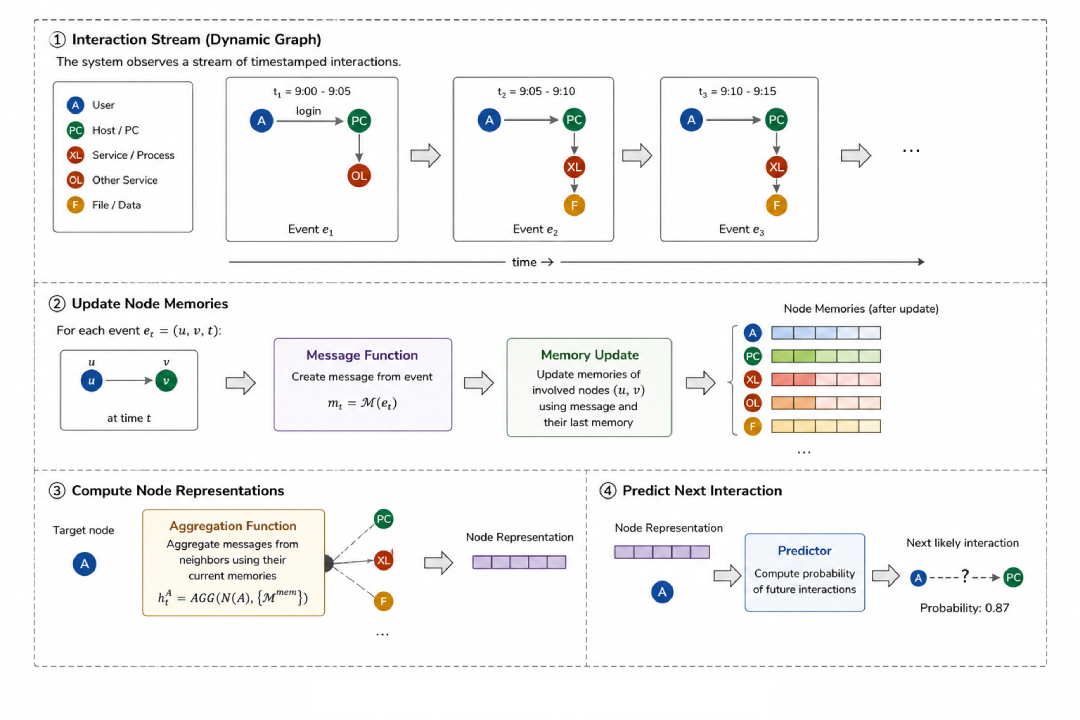
\includegraphics[width=.92\textwidth]{figures/tgn_mechanism.png}
\caption{TGN processing cycle.  A typed interaction stream produces event
messages that update per-node recurrent memory via a GRU cell.
Neighbourhood aggregation then forms node representations for next-event
prediction.  The recurrent update is both the source of temporal context
and the mutable state exposed to slow-drift poisoning.}
\label{fig:tgn}
\end{figure*}

\subsubsection{Threat model}
\label{sec:threat}

We assume an adversary who has compromised a single legitimate identity
$q$ within the monitored system.  The adversary has the following
capabilities:
\begin{itemize}
  \item \textbf{Event injection}: can issue events from $q$ to any
    endpoint that $q$ has historically communicated with, using any
    relation type observed in the training data.
  \item \textbf{Temporal control}: can choose the timing and rate of
    injected events within the pre-payload window.
  \item \textbf{Stealth objective}: seeks to minimise the anomaly score
    of a subsequent payload, not to evade the conditioning phase itself
    (which is assumed to use legitimate-looking events).
\end{itemize}

The adversary does \emph{not} have:
\begin{itemize}
  \item Access to the detector's weights, thresholds, or internal state.
  \item Ability to modify or delete existing events in the provenance
    stream.
  \item Control over multiple identities simultaneously (single-identity
    compromise).
  \item Knowledge of the defence's existence or configuration.
\end{itemize}

This threat model is conservative: the attack uses only observed event
types and templates, operating within the distribution of normal activity.
An adaptive adversary who knows the defence exists could potentially
design evasion strategies (Section~\ref{sec:future}), but the current
evaluation demonstrates that even a ``blind'' attacker using the simplest
conditioning strategy can suppress payoff scores, motivating the need
for a defence layer.

\subsubsection{The slow memory drift attack}

We distinguish two terms used throughout: a \emph{payload} is the actual
malicious activity the attacker ultimately executes (e.g.\ data
exfiltration); \emph{payoff events} $\mathcal{A}_q$ are the specific
edges whose anomaly scores the attacker seeks to suppress via
conditioning, measured to quantify the attack's effect on detection.

An adversary controls a compromised legitimate identity $q$ and issues a
conditioning sequence $\mathcal{P}$ before a fixed set of payoff events
$\mathcal{A}_q$.  The attack payoff is measured as the paired change in
anomaly score:
\begin{equation}
  \Delta_{\mathrm{pay}} = \frac{1}{|\mathcal{A}_q|}
  \sum_{e\in\mathcal{A}_q}\!
  \bigl[a_e(\mathcal{E}\cup\mathcal{P}) - a_e(\mathcal{E})\bigr].
  \label{eq:payoff}
\end{equation}
A negative $\Delta_{\mathrm{pay}}$ indicates that conditioning makes the
payload more predictable (less anomalous).  Event-level stealth is the
fraction of conditioning events that remain below the clean-validation q99
threshold:
\begin{equation}
  S_{\mathrm{evt}} = \frac{1}{|\mathcal{P}|}
  \sum_{p\in\mathcal{P}} \mathbb{1}[a_p < \tau_{.99}].
  \label{eq:stealth}
\end{equation}
A \emph{successful conditioning case} requires: (i)~high stealth
($S_{\mathrm{evt}}>0.9$), (ii)~zero pre-payload queue alerts, and
(iii)~$\Delta_{\mathrm{pay}}<0$.  This definition targets the reference
state, not end-to-end payload evasion.

\subsubsection{Four-branch difference-in-differences~\cite{angrist2009mostly}}

We isolate attack and defence effects through four paired branches that
start from an identical checkpoint and replay the same original events.
The four branches are:

\begin{center}
\begin{tabular}{cll}
\toprule
Branch & Conditioning & Defence \\
\midrule
$C$ (Clean) & absent & absent \\
$A$ (Attack) & present & absent \\
$G$ (Guard) & absent & present \\
$D$ (Defended) & present & present \\
\bottomrule
\end{tabular}
\end{center}

The Clean branch ($C$) provides a baseline.  The Attack branch ($A$) measures
what the attacker achieves without any defence.  The Guard branch ($G$)
measures the defence's cost on clean data.  The Defended branch ($D$) measures
the combined effect of attack and defence.

Defence recovery is estimated by the difference in differences:
\begin{equation}
  R = (\bar{a}_D - \bar{a}_G) - (\bar{a}_A - \bar{a}_C).
  \label{eq:did}
\end{equation}
$R>0$ means the defence reversed attacker-induced score suppression after
subtracting any clean main effect.  Bootstrap intervals~\cite{efron1979bootstrap} resample
identity-paired payoff edges.  Figure~\ref{fig:did-design} shows how the
four branches isolate causal effects.

\begin{figure}[htbp]
\centering
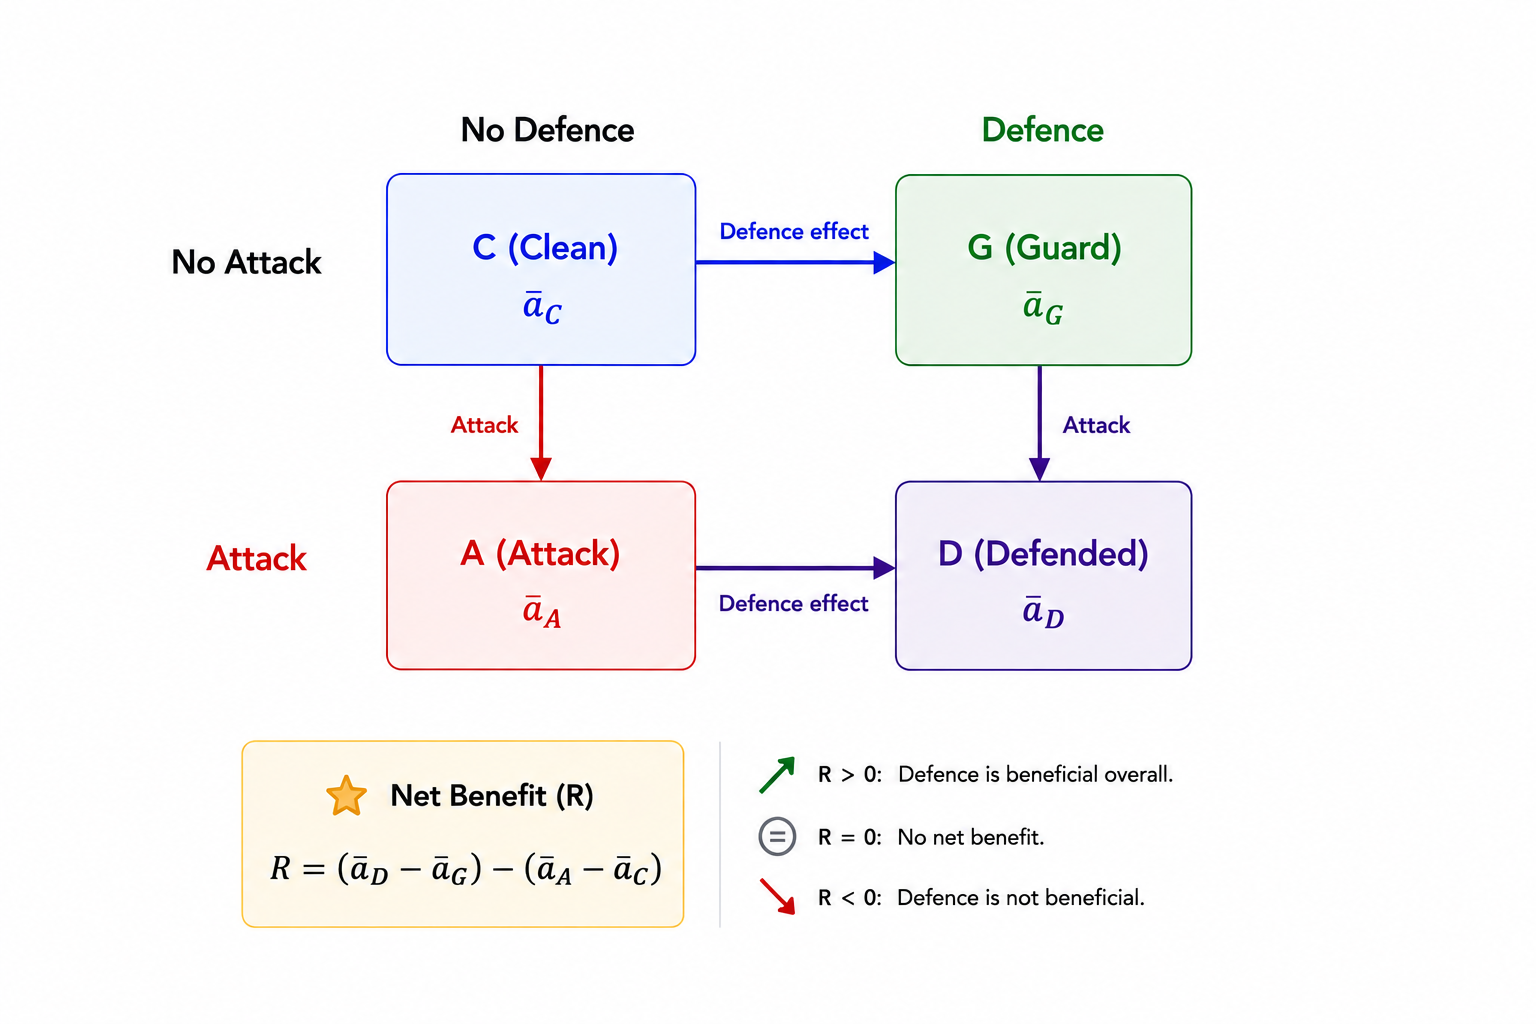
\includegraphics[width=\columnwidth]{figures/did_design_diagram.png}
\caption{Four-branch difference-in-differences design.  Each branch starts
from the same frozen checkpoint and replays the same original events.
The DiD estimator $R$ isolates the defence's causal effect on attack
suppression by subtracting any clean main effect.  $R>0$ indicates a net
benefit; $R=0$ indicates no effect; $R<0$ would indicate harm.  In all
13~experiments, $\bar{a}_C = \bar{a}_G$ exactly, so the clean main effect
is zero.}
\label{fig:did-design}
\end{figure}

\subsection{Intuition behind the proposed defence}
\label{sec:intuition}

The fundamental insight motivating this work is that slow drift attacks
exploit a \emph{trust gap} in the TGN architecture.  The model treats every
observed event as equally trustworthy for updating memory, regardless of
whether the resulting state transition is consistent with the entity's
historical role.  A process that has always communicated only with local
services should not, over dozens of events, gradually acquire a memory state
characteristic of a network-scanning tool, yet the undefended model permits
precisely this.

Our defence interposes a \emph{state-integrity gate} between the event score
and the memory commit.  The key question at each batch boundary is not
``Is this event anomalous?'' (KAIROS already answers that), but rather
``Does this event's memory update look consistent with what clean peers of
the same role produce?''

To answer this question, we extract five drift signals from each candidate
memory update.  Each signal captures a different facet of suspicious memory
evolution.  We group them into two families based on what they measure:

\paragraph{Position signals} measure whether the \emph{current state} looks
normal:
\begin{enumerate}
  \item \textbf{Role displacement}: How far has memory drifted
    from the role reference?  A large distance means the entity's
    representation no longer resembles its peers.
  \item \textbf{Event surprise}: Is the current activity itself
    suspicious to the base detector?  This is the raw anomaly score
    that KAIROS already computes.
\end{enumerate}

\paragraph{Movement signals} measure whether the \emph{pattern of state
changes} is normal:
\begin{enumerate}\setcounter{enumi}{2}
  \item \textbf{Update innovation}: Is this update unusually large
    relative to peers?  Normal updates have bounded step sizes; an
    attacker pushing memory in a specific direction may produce
    outsized steps.
  \item \textbf{Directional persistence}: Do successive updates keep
    pushing in the same direction?  Under normal operation, consecutive
    memory updates point in varying directions (a bounded random walk).
    During conditioning, updates consistently push toward the attacker's
    target (a directed walk).
  \item \textbf{Trajectory coherence}: Is the net displacement large
    relative to the total path length?  A random walk produces low
    coherence because steps cancel out~\cite{benhamou2004straightness}.
    A directed walk produces high
    coherence because steps accumulate.
\end{enumerate}

The crucial design discovery, validated experimentally in
Section~\ref{sec:interpretation}, is that \emph{movement-pattern} signals
(persistence and coherence) are far more discriminative than
\emph{position} signals for detecting gradual conditioning.  The reason is
intuitive: during conditioning, each individual step is small, so the
instantaneous state always appears normal.  But the \emph{pattern} of
changes is abnormal: ordinary memory updates resemble a bounded random
walk with low coherence and low persistence, whereas conditioning produces
sustained unidirectional drift with high coherence and high persistence.
This insight drives the optimised weight allocation that increases rate
coverage.  Figure~\ref{fig:walk-contrast} illustrates this asymmetry.

\begin{figure}[htbp]
\centering
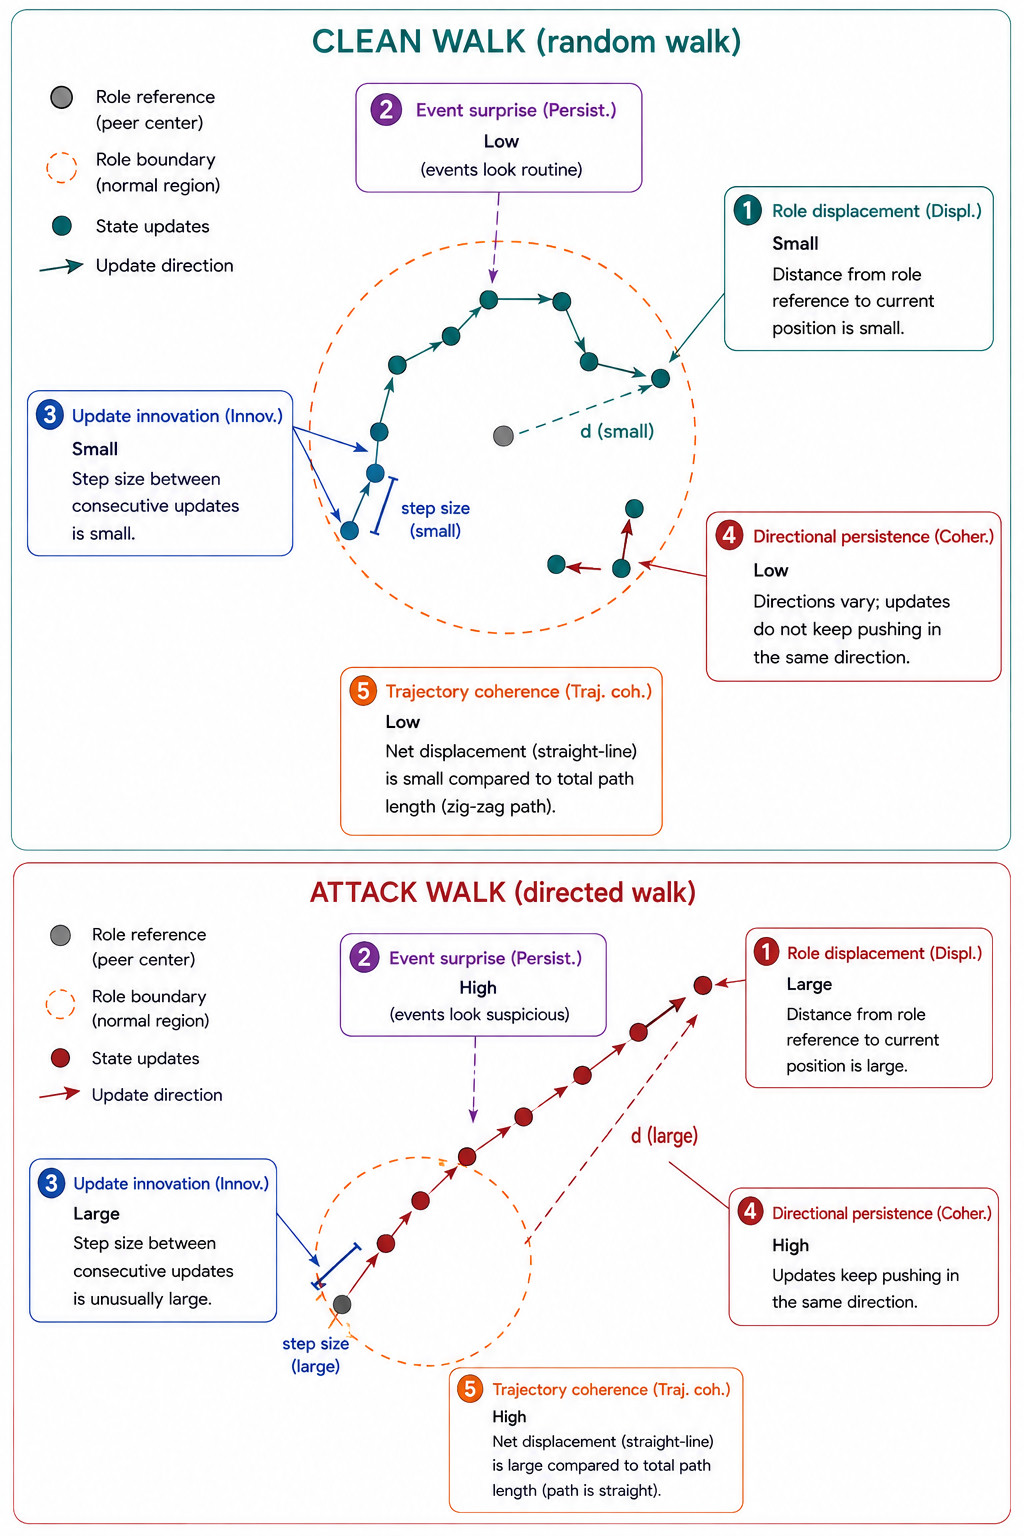
\includegraphics[width=\columnwidth]{figures/walk_contrast.jpg}
\caption{Memory trajectory contrast with drift-signal annotations.
\emph{Top}: under clean operation, consecutive updates change direction
frequently (low \textcolor{violet}{persistence}), the trajectory stays
near its origin (low \textcolor{teal!80!black}{displacement}), and the
net displacement is small relative to path length (low coherence).
\emph{Bottom}: during conditioning, updates push consistently toward the
attacker's target---small angles between steps (high
\textcolor{violet}{persistence}), large net drift from the role reference
(high \textcolor{teal!80!black}{displacement}), and net displacement
approaching total path length (high coherence).  Individual
\textcolor{orange!80!black}{innovation} (step size) may appear normal in
both cases, but the movement \emph{pattern} is distinguishable.}
\label{fig:walk-contrast}
\end{figure}

The defence is designed as a \emph{complementary} layer: it can only add
detections, never remove a KAIROS alert.  Combined alerting uses a simple
OR gate, guaranteeing that the defended system is at least as sensitive as
plain KAIROS on any input.

\subsection{Design properties of the defence}
\label{sec:properties}

The defence satisfies three structural properties by construction.
Each holds under the stated precondition; we discuss violation scenarios
inline.

\paragraph{Monotone complementarity.}  Let $\mathcal{D}_{\mathrm{KAIROS}}(e)$
denote the set of windows alerted by KAIROS and
$\mathcal{D}_{\mathrm{guard}}(e)$ the set of entities quarantined by the
guard.  The combined detection is $\mathcal{D}_{\mathrm{KAIROS}}(e) \cup
\mathcal{D}_{\mathrm{guard}}(e)$.  Since the defence never modifies KAIROS's
loss computation or queue scoring, $\mathcal{D}_{\mathrm{KAIROS}}(e)$ is
invariant to the guard's presence.  The OR gate ensures:
\begin{equation}
  |\mathcal{D}_{\mathrm{combined}}| \geq |\mathcal{D}_{\mathrm{KAIROS}}|,
  \label{eq:monotone}
\end{equation}
so the defended system can only add detections, never remove them.

\paragraph{Zero-parameter guarantee.}  The defence requires exactly zero
trainable neural parameters.  All thresholds ($h$, $k$) are derived from
order statistics of the clean-validation feature trace: $k$ is a
configurable quantile of clean evidence values, and $h$ is calibrated as
the maximum (or a high quantile) of clean CUSUM trajectories.  This means
the defence can be deployed on any frozen checkpoint without retraining.

\paragraph{Peer-isolation (precondition: single compromised identity).}
The leave-one-out construction
(Equation~\ref{eq:shrinkage}) ensures that a compromised entity cannot
influence its own peer reference.  If entity $u$ is under attack, the
role reference $\widetilde{\mathbf{m}}_{r,u}$ is computed from the
remaining $n_u - 1$ peers, none of which are under the attacker's control.
This prevents the attack from
``pulling'' its own reference toward the drift direction, which would
reduce the displacement signal and help evade detection.

\emph{Violation scenario.}  If two or more entities in the same peer
group are compromised, each attacker-controlled entity contributes to the
others' peer references.  In a peer group of size $n_u$, one compromised
entity can shift the leave-one-out median by at most one rank position.
With $c \geq 2$ compromised peers, the median can shift by up to $c-1$
ranks, progressively masking drift.  Additionally, when $n_u$ is small
(e.g.\ $n_u \ll 8$), the shrinkage toward the global median
(Equation~\ref{eq:shrinkage}) dominates the local estimate; this may
produce false positives for entities whose normal state differs
substantially from the population average.  Quantifying these boundary
conditions is left to future multi-identity evaluation.

% =====================================================================
\section{Experiments}
\label{sec:experiments}

\subsection{Defence design space}
\label{sec:design-space}

The defence pipeline has seven configurable axes.  We discuss each below,
motivate the candidate set, and summarise all candidates in
Table~\ref{tab:candidates}.

\subsubsection{Role acquisition}
\label{sec:role-acq}

Each monitored entity requires a \emph{role}, a label that groups entities
with similar expected behaviour so that peer statistics can be computed.
The choice of how to assign roles has a direct effect on the quality of the
peer reference: too broad and the reference is diluted by unrelated entities;
too narrow and the peer group is too small to produce stable statistics.

We consider three role-acquisition strategies:

\paragraph{Semantic-hash roles.}  KAIROS encodes node attributes using
hierarchical feature hashing~\cite{cheng2024kairos}, which maps filesystem
paths to vectors that preserve directory proximity (e.g., \texttt{/var/t1.txt}
is close to \texttt{/var/t2.txt}).  We can leverage this existing mechanism
to define roles: entities whose semantic-hash vectors fall within the same
cluster are assigned the same role.  This approach requires no external
metadata and is available in any KAIROS deployment, but it groups entities
by \emph{name similarity} rather than by \emph{functional behaviour}, so
two unrelated processes in the same directory would share a role even if they
perform entirely different functions.  In the CADETS evaluation, semantic
hashing reduces to executable-parent grouping because provenance entities
are identified by their process image path (Figure~\ref{fig:role-strategies}c).

\paragraph{Hierarchical LDAP roles.}  When organisational directory data
is available, roles can be structured in a hierarchy of increasing
specificity: broad role (job title), parent role (functional unit), and
fine role (department and team).  The peer reference for each entity is
computed through recursive shrinkage: each level borrows strength from
its parent when the local peer group is small.
This approach produces the tightest peer groups but requires LDAP or
equivalent directory metadata.

\paragraph{Hybrid roles.}  The hybrid strategy combines organisational
roles from LDAP with behavioural clustering derived from clean-period
activity patterns.  Behavioural features
include event-type proportions, off-hours activity fraction, weekend
activity, log event count, and unique destination ratio.  These features
are clustered using $k$-means ($k=20$), and the resulting behavioural
cluster is concatenated with the broad LDAP role to form a hybrid role
label.  This approach produces peer groups that reflect both job function
and actual system behaviour.

Figure~\ref{fig:role-strategies} shows all three role-acquisition
strategies side by side.

\begin{figure*}[!t]
\centering
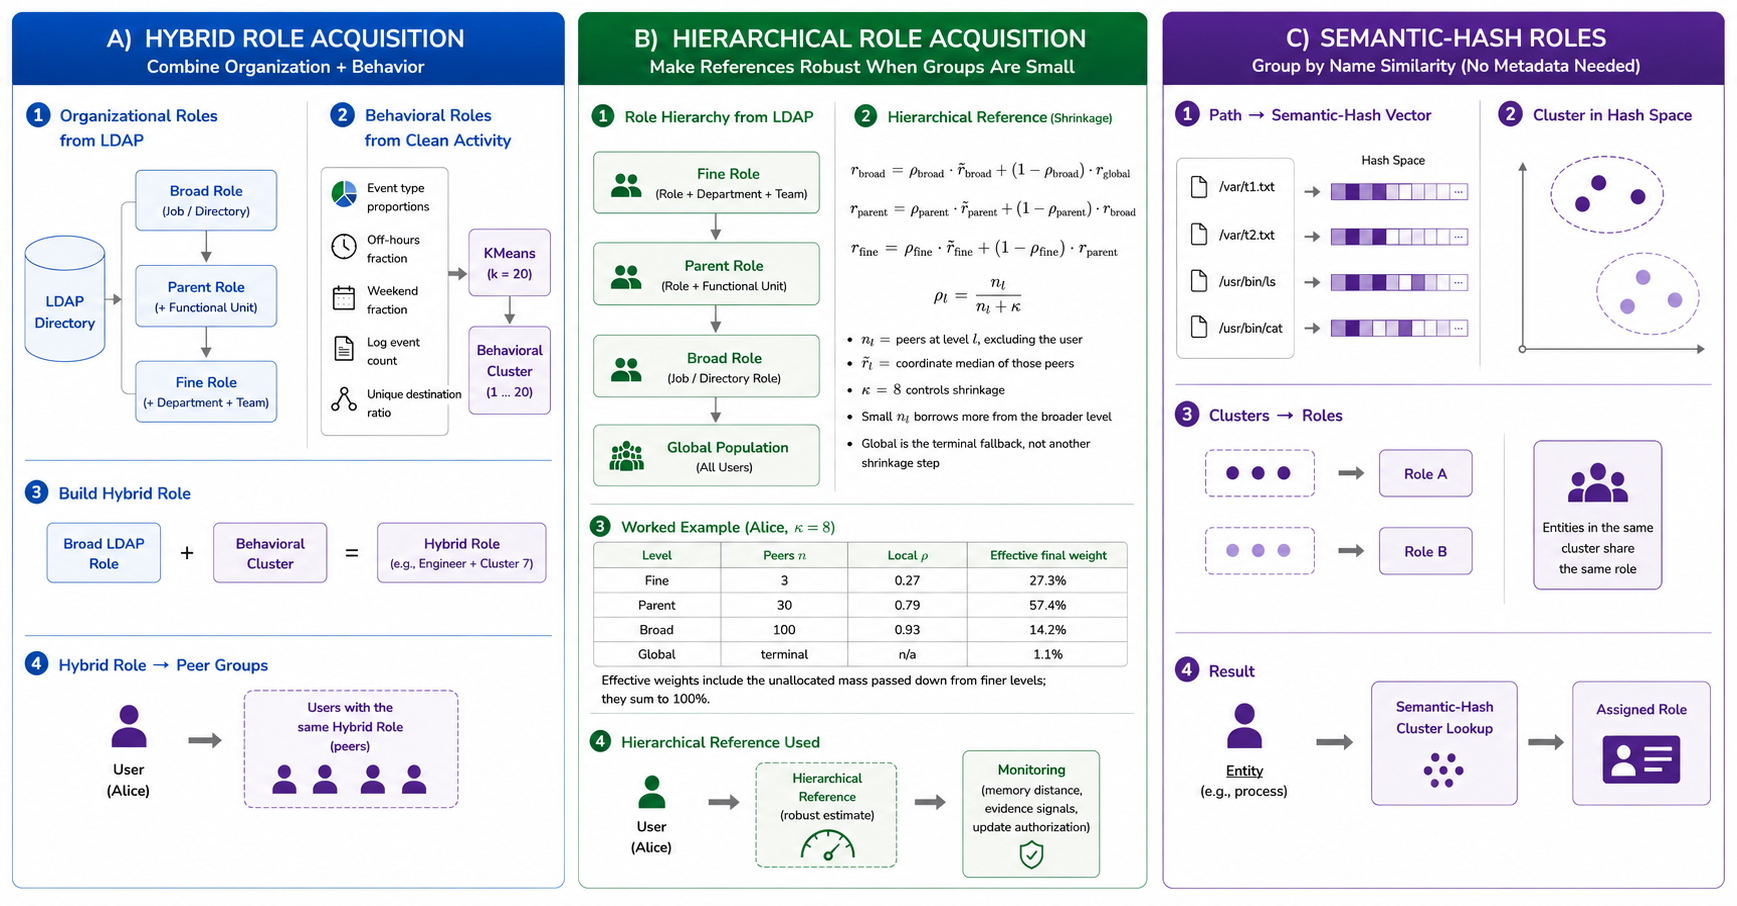
\includegraphics[width=\textwidth]{figures/role_strategies_combined.png}
\caption{Three role-acquisition strategies compared.
\textbf{(a)}~Hybrid roles concatenate the LDAP broad role with a
behavioural cluster ($k$-means on clean-period activity features),
producing groups that reflect both job function and system behaviour.
\textbf{(b)}~Hierarchical LDAP roles use a 3-level organisational hierarchy
(fine $\to$ parent $\to$ broad $\to$ global) with recursive shrinkage
($\kappa=8$); tightest peer groups but requires directory data.
\textbf{(c)}~Semantic-hash roles group entities by name similarity in hash
space---no external metadata required.}
\label{fig:role-strategies}
\end{figure*}

The CADETS dataset lacks native LDAP organisational metadata.  To enable
a controlled comparison of all three strategies on the same data, we
construct a \emph{synthetic LDAP hierarchy} that maps the 130~CADETS
subject entities to a plausible 3-level organisational structure:

\begin{itemize}
  \item \textbf{Broad} (6~departments): Platform Engineering,
    Communications, Operations, Software Engineering, File Operations,
    Security (10--29~members each).
  \item \textbf{Parent} (14~teams): e.g.\ system-core, mail-transport,
    monitoring, scripting (2--18~members each).
  \item \textbf{Fine} (34~sub-teams): e.g.\ mta-core, process-monitor,
    shell, compression (1--11~members each).
\end{itemize}

The mapping is designed to be operationally plausible: executables that
interact with similar system resources (e.g.\ \texttt{master},
\texttt{smtpd}, \texttt{qmgr} in mail-transport) are grouped together,
mirroring how LDAP directories group employees by team.  The target
entity \texttt{vUgefal} maps to dept:security $\to$ team:security-ops
$\to$ sub:unknown (5~fine peers, 10~parent peers).  This augmentation is
explicitly synthetic; its purpose is to test the \emph{mechanism} of
hierarchical shrinkage, not to claim that CADETS has organisational
structure.  Evaluation on datasets with real LDAP (e.g.\ CERT~r4.2)
is discussed in Section~\ref{sec:future}.

\subsubsection{Peer reference}

Given a role assignment, the peer reference for entity $u$ is a leave-one-out
median of role peers, shrunk toward the global median to stabilise small
groups:
\begin{align}
  \rho_u &= \frac{n_u}{n_u+\kappa}, \qquad \kappa=8, \label{eq:rho}\\
  \widetilde{\mathbf{m}}_{r,u} &= \rho_u\,\widehat{\mathbf{m}}_{r,-u}
    + (1-\rho_u)\,\widehat{\mathbf{m}}_{\mathrm{global}}.
  \label{eq:shrinkage}
\end{align}
Leave-one-out exclusion prevents a poisoned entity from pulling its own
reference toward the attack direction.  The shrinkage constant $\kappa=8$
means that a role with $n_u=8$ peers receives equal weight from local and
global estimates; smaller groups borrow more from the global reference.

\subsubsection{Distance metric}

The distance between candidate memory $\widetilde{\mathbf{s}}_u^+$ and role
reference $\mathbf{r}_u$ quantifies role displacement.  Three candidates:
\begin{itemize}
  \item \textbf{Cosine distance}: $d_{\cos}=1-\frac{\widetilde{\mathbf{s}}_u^+
    \cdot\mathbf{r}_u}{\|\widetilde{\mathbf{s}}_u^+\|_2
    \|\mathbf{r}_u\|_2}$.
    Measures directional disagreement, invariant to magnitude.
  \item \textbf{Normalised Euclidean}: $d_{\mathrm{NE}}=
    \frac{\|\widetilde{\mathbf{s}}_u^+-\mathbf{r}_u\|_2}
    {\max(\|\widetilde{\mathbf{s}}_u^+\|_2,\|\mathbf{r}_u\|_2,\epsilon)}$.
    Captures absolute separation with scale normalisation.
  \item \textbf{Diagonal robust Mahalanobis}: scales each coordinate by its
    clean-peer MAD, giving stable coordinates more weight.
\end{itemize}
Cosine is used as the primary metric in the CADETS experiments because the
official checkpoint trace was produced only with cosine distance.

\subsubsection{Evidence signals}

Five signals describe each candidate update.  With $\Delta\mathbf{s}_{u,k}
=\widetilde{\mathbf{s}}_{u,k}^+-\mathbf{s}_{u,k}^-$:
\begin{align}
  d_{r,u} &= 1 - \frac{\mathbf{m}_u^\top\widetilde{\mathbf{m}}_{r,u}}
    {\|\mathbf{m}_u\|_2\|\widetilde{\mathbf{m}}_{r,u}\|_2+\epsilon},
  & &\text{(displacement)} \nonumber\\
  I_{u,k} &= \frac{\|\Delta\mathbf{s}_{u,k}\|_2}
    {\operatorname{median}_{p\in\mathcal{R}(u)}\|\Delta\mathbf{s}_p\|_2
    +\epsilon},
  & &\text{(innovation)} \nonumber\\
  P_{u,k} &= \max\!\bigl(0,\cos(\Delta\mathbf{s}_{u,k},
    \overline{\Delta\mathbf{s}}_{u,k-1})\bigr),
  & &\text{(persistence)} \nonumber\\
  c_u(t) &= \frac{\|\sum_{j\leq t}\Delta\mathbf{m}_{u,j}\|_2}
    {\sum_{j\leq t}\|\Delta\mathbf{m}_{u,j}\|_2+\epsilon},
  & &\text{(coherence)} \nonumber\\
  a_k &= \max\text{-batch cross-entropy}.
  & &\text{(surprise)}
  \label{eq:signals}
\end{align}
Each signal is robustly standardised using clean-validation medians and
MADs~\cite{rousseeuw1993mad}:
\begin{equation}
  z_{u,t,j}^+ = \max\!\left(
    \frac{x_j-\operatorname{median}(x_{\mathrm{val},j})}
    {1.4826\operatorname{MAD}(x_{\mathrm{val},j})+\epsilon},\;0\right).
  \label{eq:robustz}
\end{equation}
The $\max(\cdot,0)$ ensures that only above-median signals contribute
evidence; normal or below-median behaviour produces zero evidence.

\subsubsection{Signal weights}

Signals are combined into scalar evidence via a weight vector
$\mathbf{w}=(w_1,\ldots,w_5)$.  Two configurations are compared:
\begin{itemize}
  \item \textbf{Original} (position-emphasising):
    $\mathbf{w}=(0.20,0.20,0.15,0.20,0.25)$.  Gives event surprise the
    largest single weight and assigns 45\% of the total to position signals
    (displacement + surprise).
  \item \textbf{Optimised} (movement-emphasising):
    $\mathbf{w}=(0.05,0.25,0.35,0.30,0.05)$.  Gives directional persistence
    and trajectory coherence a combined weight of 0.65, reducing position
    signals to 0.10.
\end{itemize}

The optimised weights were selected through a systematic grid search over
306 configurations (2~weight vectors $\times$ 3~formulas $\times$
3~monitors $\times$ 5~gap resets $\times$ 3~threshold quantiles $\times$
3~allowance quantiles), each evaluated at 4 injection rates for a total of
1,224 individual evaluations on saved feature traces.  Because the defence layer operates on pre-computed features
(not raw neural inference), this search completes in
minutes.  The results are deterministic: rerunning the search on the same
features produces identical rankings.

\subsubsection{Evidence formula}

Three formulas reduce the five weighted standardised signals to a scalar:
\begin{align}
  e^{\mathrm{mean}}_{u,t} &= \frac{\sum_j w_j z_j^+}{\sum_j w_j},
  \label{eq:mean} \\
  e^{\mathrm{max}}_{u,t} &= \max_j\!\left(w_j z_j^+\right),
  \label{eq:max} \\
  e^{\mathrm{RMS}}_{u,t} &= \sqrt{\tfrac{1}{5}\sum_j
    \left(w_j z_j^+\right)^2}.
  \label{eq:rms}
\end{align}
The weighted mean rewards consensus across signals: all five channels must
show above-normal activity for the evidence to be large.  The maximum lets
a single dominant channel drive the decision, which is useful when one
signal is strongly activated while others remain quiet.  RMS emphasises
large components without ignoring the rest, providing a middle ground.

\subsubsection{Sequential monitor}

Three monitors are compared:
\begin{itemize}
  \item \textbf{Shewhart}~\cite{shewhart1931}: alerts when a single observation exceeds
    threshold $h$.  Instantaneous; cannot accumulate weak evidence across
    multiple batches.
  \item \textbf{EMA}~\cite{roberts1959ewma}: $M_{u,t}=\alpha\,e_{u,t}+(1-\alpha)M_{u,t-1}$,
    $\alpha=0.2$.  Smooths evidence geometrically; persistent small
    excesses decay away before they can trigger an alert.
  \item \textbf{Gap-reset CUSUM}~\cite{page1954cusum}:
    $C_{u,t}=\max\{0,C_{u,t-1}+e_{u,t}-k\}$, where $k$ is the 75th
    percentile of clean evidence (the allowance).  Resets to zero after
    30~minutes of inactivity.  Alerts when $C_{u,t}>h$.
\end{itemize}
The CUSUM allowance $k$ permits ordinary fluctuation; only persistent
above-allowance evidence accumulates.  The gap reset prevents unrelated
episodes from being joined.  Threshold $h$ is calibrated as the maximum
CUSUM value observed during clean validation, ensuring zero false positives
on the calibration data.  Figure~\ref{fig:cusum-concept} illustrates how
the three monitors respond to the same evidence stream.

\begin{figure}[htbp]
\centering
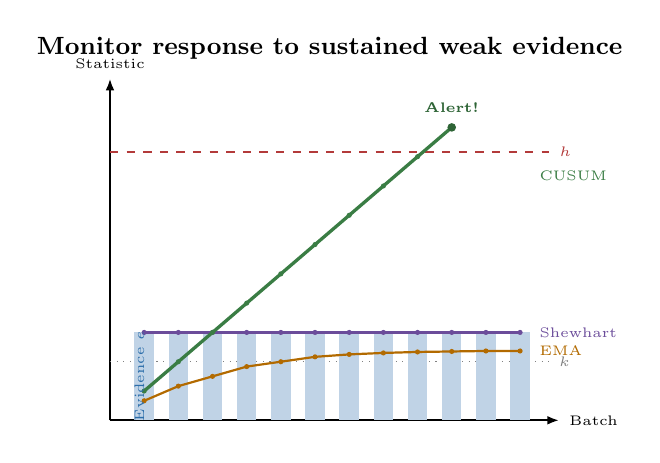
\begin{tikzpicture}[scale=0.62]
  % Title
  \node[font=\small\bfseries,anchor=south] at (4.5,7.2) {Monitor response to sustained weak evidence};
  % Axes
  \draw[-{Latex[length=1.5mm]},thick] (0,0) -- (9.2,0)
    node[right,font=\tiny] {Batch};
  \draw[-{Latex[length=1.5mm]},thick] (0,0) -- (0,7)
    node[above,font=\tiny] {Statistic};
  % Threshold line
  \draw[attackred,dashed,thick] (0,5.5) -- (9,5.5)
    node[right,font=\tiny,attackred] {$h$};
  % Allowance line
  \draw[gray,dotted] (0,1.2) -- (9,1.2)
    node[right,font=\tiny,gray] {$k$};
  % Evidence bars (small, persistent)
  \foreach \x in {0.5,1.2,1.9,2.6,3.3,4.0,4.7,5.4,6.1,6.8,7.5,8.2} {
    \fill[tgnblue!30] (\x,0) rectangle (\x+0.4,1.8);
  }
  % Shewhart (flat, never reaches h)
  \draw[purple,thick]
    (0.7,1.8) -- (1.4,1.8) -- (2.1,1.8) -- (2.8,1.8) -- (3.5,1.8)
    -- (4.2,1.8) -- (4.9,1.8) -- (5.6,1.8) -- (6.3,1.8) -- (7.0,1.8)
    -- (7.7,1.8) -- (8.4,1.8);
  \foreach \x in {0.7,1.4,2.1,2.8,3.5,4.2,4.9,5.6,6.3,7.0,7.7,8.4} {
    \fill[purple] (\x,1.8) circle (1.5pt);
  }
  \node[font=\tiny,purple,anchor=west] at (8.6,1.8) {Shewhart};
  % EMA (rises slightly then plateaus)
  \draw[amber,thick]
    (0.7,0.4) -- (1.4,0.7) -- (2.1,0.9) -- (2.8,1.1) -- (3.5,1.2)
    -- (4.2,1.3) -- (4.9,1.35) -- (5.6,1.38) -- (6.3,1.4) -- (7.0,1.41)
    -- (7.7,1.42) -- (8.4,1.42);
  \foreach \x/\y in {0.7/0.4,1.4/0.7,2.1/0.9,2.8/1.1,3.5/1.2,4.2/1.3,4.9/1.35,5.6/1.38,6.3/1.4,7.0/1.41,7.7/1.42,8.4/1.42} {
    \fill[amber] (\x,\y) circle (1.5pt);
  }
  \node[font=\tiny,amber,anchor=west] at (8.6,1.42) {EMA};
  % CUSUM (accumulates, crosses h)
  \draw[defgreen,very thick]
    (0.7,0.6) -- (1.4,1.2) -- (2.1,1.8) -- (2.8,2.4) -- (3.5,3.0)
    -- (4.2,3.6) -- (4.9,4.2) -- (5.6,4.8) -- (6.3,5.4) -- (7.0,6.0);
  \foreach \x/\y in {0.7/0.6,1.4/1.2,2.1/1.8,2.8/2.4,3.5/3.0,4.2/3.6,4.9/4.2,5.6/4.8,6.3/5.4} {
    \fill[defgreen] (\x,\y) circle (1.5pt);
  }
  \fill[defgreen!80!black] (7.0,6.0) circle (2.5pt);
  \node[font=\tiny,defgreen!80!black,anchor=south] at (7.0,6.1) {\textbf{Alert!}};
  \node[font=\tiny,defgreen,anchor=west] at (8.6,5.0) {CUSUM};
  % Evidence label
  \node[font=\tiny,tgnblue,anchor=north,rotate=90] at (0.3,0.9) {Evidence $e$};
\end{tikzpicture}
\caption{Monitor comparison on sustained weak evidence.  Each batch
produces evidence (blue bars) slightly above the allowance $k$ but well
below threshold $h$.  Shewhart tests each observation independently and
never alerts.  EMA converges to a plateau below $h$ as geometric decay
cancels accumulation.  Only CUSUM accumulates the persistent excess,
eventually crossing $h$ and triggering a guard alert.}
\label{fig:cusum-concept}
\end{figure}

\begin{table*}[!t]
\centering
\caption{Defence design matrix.  ``Compared'' entries are experimentally
varied; ``Fixed'' entries define the shared pipeline.  The total number
of candidates evaluated in the original grid is
$2\times3\times3\times5\times3\times3=810$ weight--formula--monitor--gap--threshold--allowance
cells.  After collapsing parameters unused by Shewhart and EMA monitors,
306 distinct configurations remain (Section~\ref{sec:grid}).}
\label{tab:candidates}
\resizebox{\textwidth}{!}{%
\begin{tabular}{p{.14\textwidth}p{.38\textwidth}p{.12\textwidth}p{.28\textwidth}}
\toprule
Axis & Candidates & Status & Rationale \\
\midrule
Role acquisition & Semantic-hash; functional; hierarchical LDAP; hybrid LDAP+behaviour &
  Semantic-hash & All four tested; fine-grained strategies detect only
  1 of 4 tested rates due to small CADETS peer groups
  (Table~\ref{tab:role-strategy-compare}). \\
Peer reference & Leave-one-out role median with $\kappa\!=\!8$ shrinkage &
  Fixed & Stabilises small groups; leave-one-out prevents self-contamination. \\
Distance & Cosine (primary); normalised Euclidean; diagonal Mahalanobis &
  Cosine fixed & Only cosine traced on official checkpoint. \\
Signals & Displacement, innovation, persistence, coherence, surprise &
  Fixed (5) & Separates sustained latent drift from isolated anomalous events. \\
Signal weights & Original $(0.20,0.20,0.15,0.20,0.25)$ vs.\
  optimised $(0.05,0.25,0.35,0.30,0.05)$ & Compared &
  Tests position-emphasis vs.\ movement-emphasis. \\
Evidence formula & Weighted mean, maximum, RMS &
  Compared & Tests consensus, single-channel, and energy-style aggregation. \\
Monitor & Shewhart, EMA ($\alpha\!=\!0.2$), gap-reset CUSUM &
  Compared & Tests instantaneous, smoothed, and cumulative detection. \\
Gap reset & 30, 60, 90, 120, 240 minutes &
  Compared & Controls temporal joining of unrelated episodes. \\
Threshold & Quantiles 0.99, 0.9999, 1.0 of clean validation &
  Compared & Controls false-positive rate. \\
Response & Daily-anchor rollback and quarantine until reset &
  Fixed & Ensures comparable recovery across monitors. \\
\bottomrule
\end{tabular}}
\end{table*}

\begin{figure*}[!t]
\centering
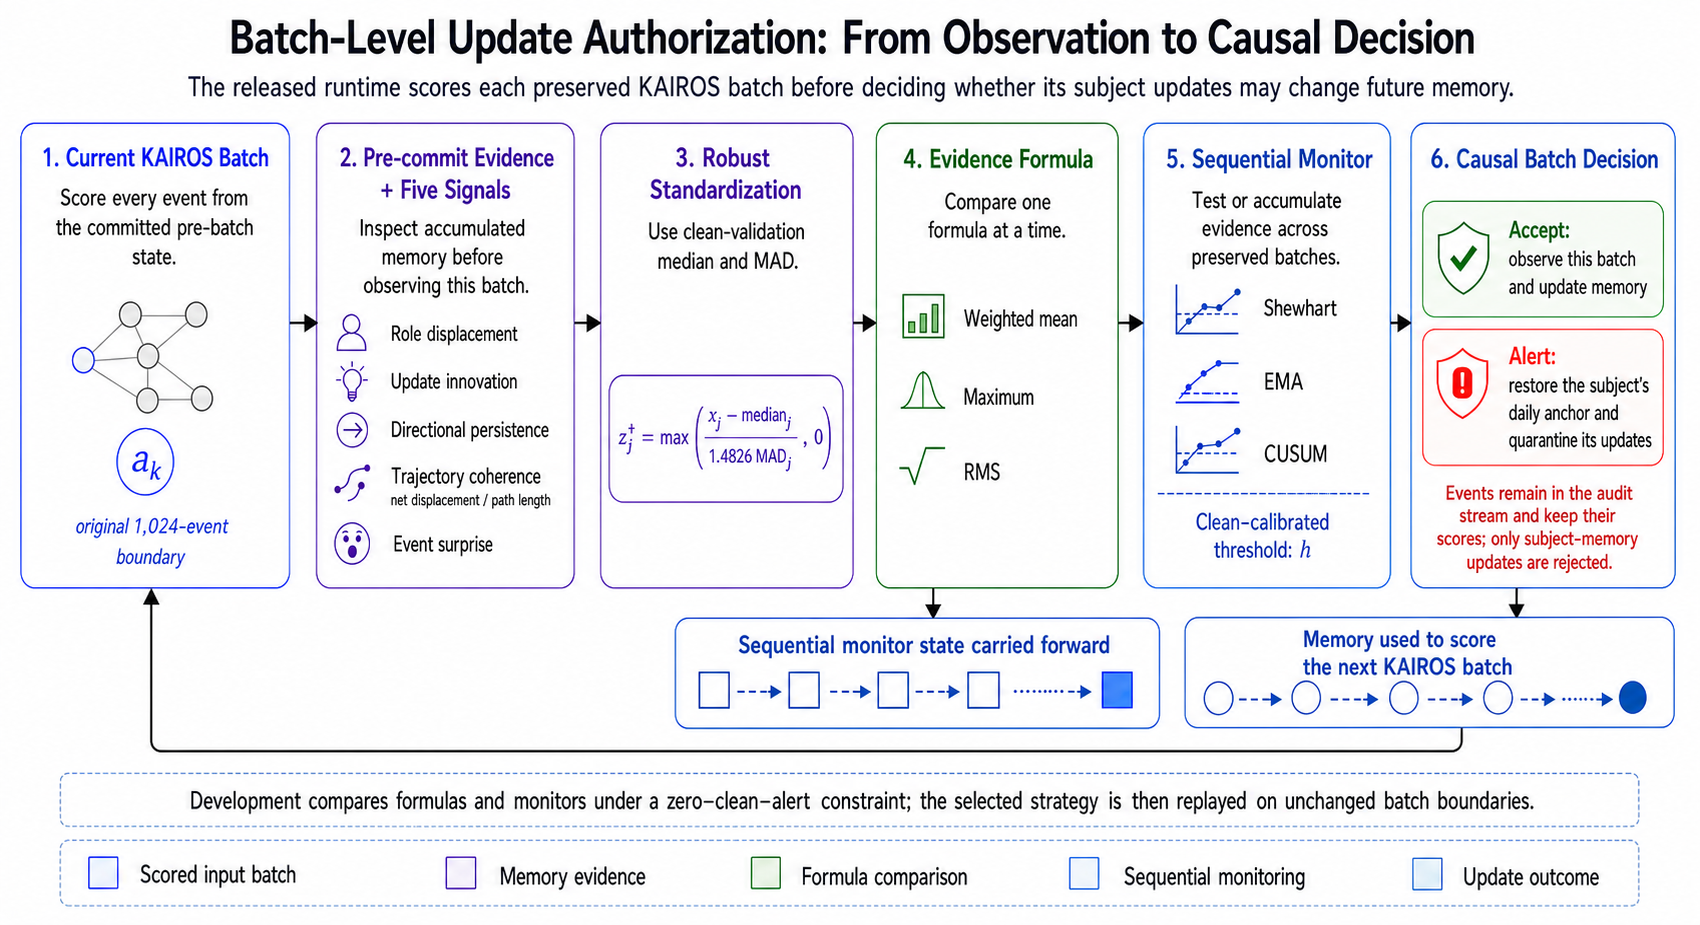
\includegraphics[width=.92\textwidth]{figures/update_authorization_pipeline_v4.png}
\caption{Implemented batch-level update-authorisation pipeline.  At each
preserved 1,024-event batch boundary, the defence extracts five signals
from the candidate memory update, robustly standardises them against
clean-validation medians and MADs, combines them via the selected evidence
formula, and feeds the result into the sequential monitor.  If the monitor
statistic exceeds its threshold, the subject entity's memory is restored
to a daily anchor and subsequent updates are quarantined (rejected).
Events remain visible and scored in both the accept and alert paths;
only the subject's \emph{memory updates} are blocked.}
\label{fig:pipeline}
\end{figure*}

\subsection{Experimental protocol}
\label{sec:protocol}

\subsubsection{Dataset and base detector}
\label{sec:datasets}

\paragraph{DARPA CADETS~E3 (conditioning evaluation).}
The slow-conditioning attack and defence configuration search use the
released KAIROS CADETS~E3~\cite{darpa2018tc} checkpoint
(\texttt{cadets3\_models.pt}) without training or fine-tuning.  The official
chronology is preserved: days~3--5 fit clean-reference statistics and
candidate thresholds; day~6 contains the released attack and receives
synthetic conditioning; day~7 is an out-of-sample clean control (2,284,034
events).  All neural weights, IDF values, queue boundaries, and attack
labels remain frozen.  The baseline reproduction yields TN\,=\,174,
FP\,=\,1, FN\,=\,0, TP\,=\,4 (precision 0.80, recall 1.00, F1 0.89).

Using a single frozen checkpoint is a deliberate methodological choice:
it ensures that every experimental branch starts from an identical state,
making the four-branch DiD design internally valid.

\paragraph{CMU CERT~r4.2 (multi-target longitudinal evaluation).}
To evaluate the defence across diverse insiders, attack scenarios, and
temporal positions, we train five independent TGN checkpoints (seeds 17,
29, 43, 59, 71) on the CMU CERT~r4.2 insider-threat
corpus~\cite{lindauer2020cert} using the adapted KAIROS
architecture~\cite{cheng2024kairos}.  The corpus spans 1,000~users across
an 18-month period (January~2010--May~2011) with 15.6~million events.
Ground truth comprises \textbf{70~labelled insiders} across three scenarios:
\begin{itemize}
  \item \textbf{Scenario~1} (30~insiders): USB exfiltration to a
    competitor, 5--20 target-actor events per case;
  \item \textbf{Scenario~2} (30~insiders): data theft via thumb drive
    uploads, 192--267 target-actor events spanning weeks;
  \item \textbf{Scenario~3} (10~insiders): sysadmin keylogger
    deployment with a confederate, 12--20 target-actor events across a
    2-day attack window.
\end{itemize}
The three high-quality checkpoints (seeds 17, 59, 71) achieve validation
reconstruction error $\leq 0.055$ and edge-type accuracy $\geq 97.6\%$;
the two lower-quality checkpoints (seeds 29, 43) have validation error
$\approx 0.10$ and accuracy $\approx 95.6\%$.  Including all five seeds
tests whether the defence is robust to checkpoint quality variation.
All 19~defence configurations (6~role strategies $\times$ 3~reference
methods $+$ primary) are evaluated on the full 70-insider corpus across
5~seeds, yielding \textbf{6,650 case-level evaluations}.

\subsubsection{Attack construction}

The compromised subject is the real CADETS process \texttt{vUgefal}.
Conditioning events use the clean-validation-observed relation
\texttt{EVENT\_RECVFROM} with endpoint \texttt{128.55.12.10:53}, supported
by 3,524 matching validation events.  Injected events are merged into their
temporally correct 1,024-event batches without displacing original events.
Twelve injection rates are tested: 1, 2, 3, 4, 6, 8, 10, 15, 20, 30, 50,
and 100 interactions per hour, beginning at 00:05 on day~6 and ending
before the official 11:18 payload.  The original four rates (1, 4, 20, 100)
were used for configuration search; eight additional rates (2, 3, 6, 8, 10,
15, 30, 50) map the detection boundary.

A secondary stressor uses the reverse \texttt{EVENT\_SENDTO} relation at
20 events per hour to test cross-relation robustness.

The CADETS conditioning evaluation uses a single target entity on a single
attack day, ensuring internal validity of the four-branch DiD design but
limiting external generalisability.  The complementary CERT~r4.2
longitudinal evaluation (Section~\ref{sec:multi-target}) tests the same
defence signals and monitor across 70~labelled insiders, 3~attack
scenarios, 10~months of events, and 5~independently trained checkpoints,
providing the multi-target breadth that the CADETS design lacks.

\subsubsection{Evaluation gates}

The defence is judged through three scoped gates:
\begin{enumerate}
  \item \textbf{Clean cost}: no increase in alerted queue windows on the
    clean day; report guard alerts and quarantined updates on both the
    clean paired branch ($G$) and out-of-sample day~7.  Specifically,
    we require $\bar{a}_C = \bar{a}_G$ to machine precision across
    all tested rates.
  \item \textbf{Detection parity}: preserve KAIROS's four attack-window
    detections and its existing false positive.  The defence must not
    interfere with any existing KAIROS decision.
  \item \textbf{Conditioning detection}: guard alerts before payload
    arrival; $R>0$ with identity-paired payoff edges; report the number
    of injection rates detected (rate coverage) out of the 12 tested.
\end{enumerate}

\subsubsection{Threshold calibration}

The CUSUM threshold $h$ and allowance $k$ are calibrated from the
clean-validation feature trace, a saved \texttt{.npz} file containing
the five drift signals computed on the day~3--5 validation data.  The
grid sweep tested three quantile levels for each:

\begin{itemize}
  \item \textbf{Threshold quantile} $q_h \in \{0.99, 0.9999, 1.0\}$:
    controls the maximum CUSUM value tolerated on clean data.  $q_h = 1.0$
    (the clean maximum) produces the tightest possible threshold at zero
    false positives.  Lower quantiles admit more aggressive detection but
    risk false positives on extreme clean observations.
  \item \textbf{Allowance quantile} $q_k \in \{0.50, 0.75, 0.90\}$:
    controls how much ordinary fluctuation is ``forgiven'' before evidence
    accumulates.  $q_k = 0.75$ means the CUSUM only counts the excess
    above the 75th percentile of clean evidence; lower quantiles make the
    monitor more sensitive but also more prone to accumulating noise.
\end{itemize}

The winning configuration uses $q_h = 1.0$ and $q_k = 0.75$, yielding
$h = 302.01$ and $k = 1.030$.  This combination maximises rate coverage
at exactly zero false positives.  Lowering $q_h$ to $0.9999$ produces
the same rate coverage but risks non-zero FP on rare clean extremes.
Lowering $q_k$ to $0.50$ detects one additional rate in the grid search
but introduces false positives on entities with naturally variable
behaviour.


% =====================================================================
\section{Results}
\label{sec:results}

\subsection{The base detector is blind to conditioning}

Table~\ref{tab:attack} reports the undefended base detector's response to
the conditioning phase.  At every tested injection rate, the conditioning
is invisible to KAIROS: zero queue alerts across all 43 pre-payload windows.
Event-level stealth (the fraction of conditioning events that score below
the clean q99 threshold) ranges from 91.7\% at rate~1 to 99.8\% at
rate~100 (Figure~\ref{fig:event-stealth}).  All four official payload
windows remain detected (recall\,=\,1.0).

The attack therefore achieves \emph{pre-payload blindness with score
suppression}, not full payload evasion.  The conditioning makes the target
entity's future events more predictable (lower anomaly scores) without
triggering any alert during the conditioning period itself.

\begin{table}[htbp]
\centering
\caption{Attack stealth and payoff suppression across 12 injection rates.
Plain KAIROS detects zero conditioning windows at all 12 tested rates.
$\Delta_{\mathrm{pay}}$ is the mean paired change in anomaly score for
specific-payoff edges (Equation~\ref{eq:payoff}); negative values
indicate score suppression.  The pre-payload alert column counts the number of
conditioning-phase queue windows that KAIROS flags out of 43 total.
The conditioning phase is invisible to the base detector across two
orders of magnitude of injection intensity.}
\label{tab:attack}
\resizebox{\columnwidth}{!}{%
\begin{tabular}{rrrc}
\toprule
Rate (/hr) & Events & $\Delta_{\mathrm{pay}}$ &
  Pre-payload alerts \\
\midrule
1   & 12    & $-0.00350$ & 0\,/\,43 \\
2   & 23    & $-0.00354$ & 0\,/\,43 \\
3   & 34    & $-0.00352$ & 0\,/\,43 \\
4   & 45    & $-0.00356$ & 0\,/\,43 \\
6   & 67    & $-0.00353$ & 0\,/\,43 \\
8   & 90    & $-0.00355$ & 0\,/\,43 \\
10  & 112   & $-0.00354$ & 0\,/\,43 \\
15  & 168   & $-0.00357$ & 0\,/\,43 \\
20  & 223   & $-0.00354$ & 0\,/\,43 \\
30  & 335   & $-0.00358$ & 0\,/\,43 \\
50  & 558   & $-0.00355$ & 0\,/\,43 \\
100 & 1,115 & $-0.00352$ & 0\,/\,43 \\
\bottomrule
\end{tabular}}
\end{table}

\begin{figure}[htbp]
\centering
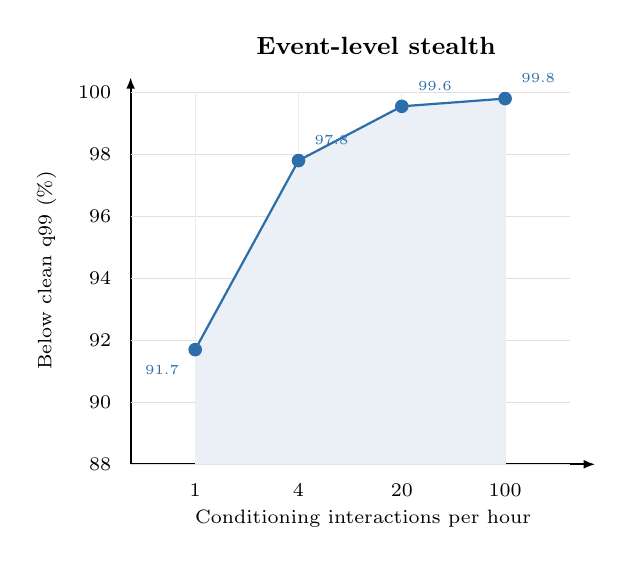
\begin{tikzpicture}[scale=0.82]
  % Title
  \node[font=\small\bfseries,anchor=south] at (3.8,6.2) {Event-level stealth};
  % Axes
  \draw[-{Latex[length=1.5mm]},thick] (0,0) -- (7.2,0);
  \node[font=\scriptsize,anchor=north] at (3.6,-0.55) {Conditioning interactions per hour};
  \draw[-{Latex[length=1.5mm]},thick] (0,0) -- (0,6.0);
  \node[font=\scriptsize,rotate=90,anchor=south] at (-1.0,3.0) {Below clean q99 (\%)};
  % Y-axis: range 88–101, each unit = 0.48cm (more vertical space)
  \def\ybase{88}
  \def\yscale{0.48}
  \foreach \v in {88,90,92,94,96,98,100} {
    \pgfmathsetmacro{\yy}{(\v-\ybase)*\yscale}
    \draw[gray!25,thin] (0,\yy) -- (6.8,\yy);
    \node[font=\scriptsize,anchor=east] at (-0.15,\yy) {\v};
  }
  % X-axis: log-ish spacing for 1, 4, 20, 100
  \def\xa{1.0}   % rate 1
  \def\xb{2.6}   % rate 4
  \def\xc{4.2}   % rate 20
  \def\xd{5.8}   % rate 100
  \foreach \x/\lab in {\xa/1, \xb/4, \xc/20, \xd/100} {
    \node[font=\scriptsize,anchor=north] at (\x,-0.15) {\lab};
    \draw[gray!15,thin] (\x,0) -- (\x,{(100-\ybase)*\yscale});
  }
  % Data: stealth = 91.7, 97.8, 99.6, 99.8
  \pgfmathsetmacro{\ya}{(91.7-\ybase)*\yscale}
  \pgfmathsetmacro{\yb}{(97.8-\ybase)*\yscale}
  \pgfmathsetmacro{\yc}{(99.55-\ybase)*\yscale}
  \pgfmathsetmacro{\yd}{(99.8-\ybase)*\yscale}
  % Shaded area under curve
  \fill[tgnblue!10] (\xa,0) -- (\xa,\ya) -- (\xb,\yb) -- (\xc,\yc)
    -- (\xd,\yd) -- (\xd,0) -- cycle;
  % Line
  \draw[tgnblue,thick] (\xa,\ya) -- (\xb,\yb) -- (\xc,\yc) -- (\xd,\yd);
  % Dots with value labels
  \fill[tgnblue] (\xa,\ya) circle (3pt);
  \node[font=\tiny,tgnblue,anchor=north east] at (\xa-0.1,\ya-0.1) {91.7};
  \fill[tgnblue] (\xb,\yb) circle (3pt);
  \node[font=\tiny,tgnblue,anchor=south west] at (\xb+0.1,\yb+0.1) {97.8};
  \fill[tgnblue] (\xc,\yc) circle (3pt);
  \node[font=\tiny,tgnblue,anchor=south west] at (\xc+0.1,\yc+0.1) {99.6};
  \fill[tgnblue] (\xd,\yd) circle (3pt);
  \node[font=\tiny,tgnblue,anchor=south west] at (\xd+0.1,\yd+0.1) {99.8};
\end{tikzpicture}
\caption{Event-level stealth of the conditioning attack.  The fraction
of injected events scoring below the clean q99 threshold increases with
rate: from 91.7\% at rate~1 to 99.8\% at rate~100.  Even at the lowest
rate, over 90\% of conditioning events are individually indistinguishable
from clean traffic, confirming that per-event anomaly scores cannot
detect slow drift.}
\label{fig:event-stealth}
\end{figure}

\subsection{Full configuration grid}
\label{sec:grid}

We evaluated \textbf{306 configurations} (2~weight vectors $\times$
3~formulas $\times$ 3~monitors $\times$ 5~gap resets $\times$ 3~threshold
quantiles $\times$ 3~allowance quantiles), each tested on four representative
injection rates (1, 4, 20, 100~events/hour), for a total of
\textbf{1,224 individual evaluations}.  Table~\ref{tab:grid-summary}
reports the full breakdown.

Of the 306 configurations, 154 produce zero false positives on the
clean day~7 trace (19,464 batch records, 87 unique nodes).  The remaining
152 produce between 1 and 510 false-positive alerts.

\begin{table}[htbp]
\centering
\caption{Strategy ranking by detection coverage across all 12~attack rates
(1--100~events/hr).  The winning configuration was evaluated at all
12~rates; other strategies were screened during the 4-rate grid sweep
(rates~1, 4, 20, 100) and their 12-rate coverage is a conservative lower
bound ($\geq$).  All listed strategies produce zero false positives on the
out-of-sample clean trace unless noted.}
\label{tab:grid-summary}
\resizebox{\columnwidth}{!}{%
\begin{tabular}{lcc}
\toprule
Strategy & Rates detected (/12) & Clean FP \\
\midrule
Max + CUSUM, opt.\ wts, flat semantic
  & \textbf{7/12} & 0 \\
CUSUM + opt.\ wts (grid best, 32~configs)
  & $\geq$\,3/12$^*$ & 0 \\
CUSUM + original wts
  & $\geq$\,1/12$^*$ & 0 \\
Functional role strategy
  & $\geq$\,1/12$^*$ & 0 \\
Hierarchical role strategy
  & $\geq$\,1/12$^*$ & 0 \\
Hybrid role strategy
  & $\geq$\,1/12$^*$ & 0 \\
Shewhart (all zero-FP configs)
  & 0/12 & 0 \\
EMA (all zero-FP configs)
  & 0/12 & 0 \\
\midrule
Plain KAIROS (baseline)
  & 0/12 & --- \\
\bottomrule
\end{tabular}}

\smallskip
{\footnotesize $^*$Evaluated at 4~grid rates only;
12-rate coverage is a lower bound.}
\end{table}

Figure~\ref{fig:grid-bars} ranks every strategy family by detection
coverage on the full 12-rate scale.

\begin{figure}[htbp]
\centering
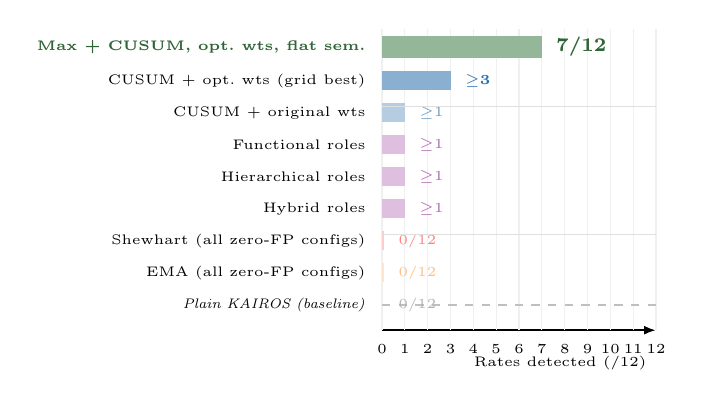
\begin{tikzpicture}[scale=0.58]
  % Comprehensive ranked leaderboard — horizontal bars, /12 scale
  \def\bh{0.42}          % bar height
  \def\rs{0.50}          % x-scale: 0.50 cm per rate
  \def\ysp{0.70}         % row spacing
  \pgfmathsetmacro{\xmax}{\rs*12}
  \pgfmathsetmacro{\ytop}{9*\ysp+0.3}
  % --- Axes ---
  \draw[-{Latex[length=1.5mm]},thick] (0,0) -- (\xmax,0);
  \node[font=\tiny,anchor=north east] at (\xmax,-0.35)
    {Rates detected (/12)};
  \draw[thick] (0,0) -- (0,\ytop);
  % X-axis ticks 0–12
  \foreach \v in {0,1,...,12} {
    \pgfmathsetmacro{\xpos}{\v*\rs}
    \draw[gray!12,thin] (\xpos,0) -- (\xpos,\ytop);
    \node[font=\tiny,anchor=north] at (\xpos,-0.1) {\v};
  }
  % --- Rows (bottom to top, worst to best) ---
  % Row 1: Plain KAIROS baseline (dashed line)
  \pgfmathsetmacro{\yb}{0.35}
  \draw[dashed,gray!50,thick] (0,\yb+\bh/2) -- (\xmax,\yb+\bh/2);
  \node[font=\tiny,anchor=east] at (-0.15,\yb+\bh/2)
    {\textit{Plain KAIROS (baseline)}};
  \node[font=\tiny,gray!60,anchor=west] at (0.15,\yb+\bh/2) {0/12};
  % Row 2: EMA zero-FP
  \pgfmathsetmacro{\yb}{0.35+\ysp}
  \fill[orange!20] (0,\yb) rectangle (0.04,\yb+\bh);
  \node[font=\tiny,anchor=east] at (-0.15,\yb+\bh/2)
    {EMA (all zero-FP configs)};
  \node[font=\tiny,orange!50,anchor=west] at (0.15,\yb+\bh/2) {0/12};
  % Row 3: Shewhart zero-FP
  \pgfmathsetmacro{\yb}{0.35+2*\ysp}
  \fill[red!20] (0,\yb) rectangle (0.04,\yb+\bh);
  \node[font=\tiny,anchor=east] at (-0.15,\yb+\bh/2)
    {Shewhart (all zero-FP configs)};
  \node[font=\tiny,red!50,anchor=west] at (0.15,\yb+\bh/2) {0/12};
  \draw[gray!25,thin] (0,0.35+2.5*\ysp) -- (\xmax,0.35+2.5*\ysp);
  % Row 4: Hybrid roles (≥1/12)
  \pgfmathsetmacro{\yb}{0.35+3*\ysp}
  \fill[violet!25] (0,\yb) rectangle (\rs,\yb+\bh);
  \node[font=\tiny,anchor=east] at (-0.15,\yb+\bh/2) {Hybrid roles};
  \node[font=\tiny,violet!60,anchor=west] at (\rs+0.1,\yb+\bh/2)
    {$\geq$1};
  % Row 5: Hierarchical roles (≥1/12)
  \pgfmathsetmacro{\yb}{0.35+4*\ysp}
  \fill[violet!25] (0,\yb) rectangle (\rs,\yb+\bh);
  \node[font=\tiny,anchor=east] at (-0.15,\yb+\bh/2)
    {Hierarchical roles};
  \node[font=\tiny,violet!60,anchor=west] at (\rs+0.1,\yb+\bh/2)
    {$\geq$1};
  % Row 6: Functional roles (≥1/12)
  \pgfmathsetmacro{\yb}{0.35+5*\ysp}
  \fill[violet!25] (0,\yb) rectangle (\rs,\yb+\bh);
  \node[font=\tiny,anchor=east] at (-0.15,\yb+\bh/2)
    {Functional roles};
  \node[font=\tiny,violet!60,anchor=west] at (\rs+0.1,\yb+\bh/2)
    {$\geq$1};
  % Row 7: CUSUM + original wts (≥1/12)
  \pgfmathsetmacro{\yb}{0.35+6*\ysp}
  \fill[tgnblue!35] (0,\yb) rectangle (\rs,\yb+\bh);
  \node[font=\tiny,anchor=east] at (-0.15,\yb+\bh/2)
    {CUSUM + original wts};
  \node[font=\tiny,tgnblue!70,anchor=west] at (\rs+0.1,\yb+\bh/2)
    {$\geq$1};
  \draw[gray!25,thin] (0,0.35+6.5*\ysp) -- (\xmax,0.35+6.5*\ysp);
  % Row 8: CUSUM + opt wts grid best (≥3/12)
  \pgfmathsetmacro{\yb}{0.35+7*\ysp}
  \fill[tgnblue!55] (0,\yb) rectangle (3*\rs,\yb+\bh);
  \node[font=\tiny,anchor=east] at (-0.15,\yb+\bh/2)
    {CUSUM + opt.\ wts (grid best)};
  \node[font=\tiny\bfseries,tgnblue,anchor=west] at (3*\rs+0.1,\yb+\bh/2)
    {$\geq$3};
  % Row 9: Winner — Max + CUSUM opt wts (7/12)
  \pgfmathsetmacro{\yb}{0.35+8*\ysp}
  \fill[defgreen!55] (0,\yb) rectangle (7*\rs,\yb+\bh+0.08);
  \node[font=\tiny\bfseries,anchor=east] at (-0.15,\yb+\bh/2+0.04)
    {\textcolor{defgreen!80!black}{Max + CUSUM, opt.\ wts, flat sem.}};
  \node[font=\scriptsize\bfseries,defgreen!80!black,anchor=west]
    at (7*\rs+0.1,\yb+\bh/2+0.04) {7/12};
\end{tikzpicture}
\caption{Comprehensive strategy ranking by detection coverage on all
12~attack rates (1--100~events/hr), zero false positives.  Strategies
below the dashed baseline offer no improvement over plain KAIROS.
Role strategies and grid-sweep configurations ($\geq$) were evaluated at
4~representative rates; 12-rate coverage is a lower bound.  The winning
configuration (top bar) was evaluated across all 12~rates.}
\label{fig:grid-bars}
\end{figure}

Three structural findings emerge from the sweep:

\paragraph{CUSUM is the only effective monitor at zero FP.}
All zero-FP Shewhart and EMA configurations detect 0/12~rates.  Every
detection at zero FP comes from CUSUM.  Shewhart and EMA can reach 4/12,
but only by accepting 165+ false-positive records (34--67 clean nodes
alerted).

\paragraph{Movement-emphasis weights unlock rate coverage.}
Among the 154 zero-FP configurations, the 75 using original weights achieve
a maximum of 1/12~rates, while the 79 using optimised weights achieve a
maximum of 3/12~rates at the 4-rate grid level.  When the best optimised-weight
configuration is extended to all 12~rates, it detects 7/12
(Section~\ref{sec:weight-opt}).

\paragraph{No zero-FP configuration detects rate~1.}
Across all 306 configurations, rate~1 is detected only with thresholds that
produce 165+ false positives.  This is a structural floor, not a tuning gap
(see Section~\ref{sec:interpretation}).

\subsection{Weight optimisation: from 1/12 to 7/12 rate coverage}
\label{sec:weight-opt}

The grid sweep confirms that \textbf{movement-emphasis weights dramatically
improve rate coverage}.  Table~\ref{tab:weight-comparison} summarises the
comparison between the two weight vectors.

\begin{table}[htbp]
\centering
\caption{Weight optimisation impact on rate coverage.  Both configurations
are evaluated on the same 12 injection rates (1--100~events/hr).
The movement-emphasis configuration (persistence + coherence = 0.65)
increases detection from 1/12 to 7/12 compared to the position-emphasis
configuration (displacement + surprise = 0.45).  Both produce zero clean
false positives.}
\label{tab:weight-comparison}
\resizebox{\columnwidth}{!}{%
\begin{tabular}{lccc}
\toprule
Configuration & Coverage (/12) & Clean FP & Detected rates \\
\midrule
Original $(0.20,0.20,0.15,0.20,0.25)$ & 1/12 & 0 & 20 only \\
\textbf{Optimised} $\mathbf{(0.05,0.25,0.35,0.30,0.05)}$ &
  \textbf{7/12} & \textbf{0} & \textbf{4, 10, 15, 20, 30, 50, 100} \\
\bottomrule
\end{tabular}}
\end{table}

\subsection{The winning strategy}
\label{sec:winner}

\subsubsection{Configuration summary}

The winning strategy is:
\begin{itemize}
  \item \textbf{Evidence formula}: maximum positive evidence
    ($e^{\mathrm{max}}$, Equation~\ref{eq:max}), which lets the single
    strongest signal channel drive the evidence score.
  \item \textbf{Sequential monitor}: gap-reset CUSUM with 30-minute gap
    reset, allowance $k=1.030$ (75th percentile of clean evidence),
    and threshold $h=302.01$ (maximum observed in clean validation).
  \item \textbf{Signal weights}: $(0.05,0.25,0.35,0.30,0.05)$, assigning
    65\% of the total weight to movement-pattern signals (persistence +
    coherence) and only 10\% to position signals (displacement + surprise).
\end{itemize}

This configuration outperforms all 153 zero-FP alternatives on rate
coverage, detecting conditioning at 7 of 12 tested rates with zero false
positives.
The RMS formula achieves identical rate coverage but with slightly later
alert times.  The weighted-mean formula detects only 1 of 4 rates with
optimised weights, because the consensus requirement dilutes the signal
from the dominant channel.

\subsubsection{Primary results: 12-rate detection boundary}

Table~\ref{tab:primary} presents the full four-branch results with
optimised weights across \textbf{12 injection rates} spanning two orders
of magnitude (1--100~events/hour).  Each rate was evaluated using the
complete four-branch DiD protocol.

\begin{table*}[!t]
\centering
\caption{Defence performance with optimised weights across 12 injection
rates.  The defended system detects conditioning at 7 of 12 rates with
zero false positives.  A non-monotonic gap appears at rates~6 and~8
(Section~\ref{sec:nonmono}).  Recovery $R$ is the paired DiD
(Equation~\ref{eq:did}) on specific-payoff edges.  All detected rates
produce identical $R=+0.135$ because the quarantine mechanism is binary.
Clean effect $= 0.0000$ in every row, confirming zero defence cost.}
\label{tab:primary}
\resizebox{\textwidth}{!}{%
\begin{tabular}{rrcccrrl}
\toprule
Rate (/hr) & Events & Detected & Quarantine (\%) &
  Lead time (h) & $R$ (specific) & 95\% CI & Clean FP (day 7) \\
\midrule
1   & 12    & No  & ---  & ---  & 0.0    & --- & 0 \\
2   & 23    & No  & ---  & ---  & 0.0    & --- & 0 \\
3   & 34    & No  & ---  & ---  & 0.0    & --- & 0 \\
4   & 45    & \textbf{Yes} & 13.3  & 1.5  & +0.1354 &
  $[+0.113,\;+0.160]$ & 0 \\
6   & 67    & No  & ---  & ---  & 0.0    & --- & 0 \\
8   & 90    & No  & ---  & ---  & 0.0    & --- & 0 \\
10  & 112   & \textbf{Yes} & 9.8  & 1.1  & +0.1354 &
  $[+0.113,\;+0.160]$ & 0 \\
15  & 168   & \textbf{Yes} & 39.9  & 4.5  & +0.1354 &
  $[+0.113,\;+0.160]$ & 0 \\
20  & 223   & \textbf{Yes} & 82.5  & 9.3  & +0.1354 &
  $[+0.113,\;+0.159]$ & 0 \\
30  & 335   & \textbf{Yes} & 69.9  & 7.9  & +0.1354 &
  $[+0.113,\;+0.160]$ & 0 \\
50  & 558   & \textbf{Yes} & 67.7  & 7.6  & +0.1354 &
  $[+0.113,\;+0.160]$ & 0 \\
100 & 1,115 & \textbf{Yes} & 88.3  & 9.9  & +0.1354 &
  $[+0.112,\;+0.160]$ & 0 \\
\bottomrule
\end{tabular}}
\end{table*}

The detection boundary reveals three regimes:
\begin{enumerate}
  \item \textbf{Below floor} (rates 1--3, $\leq$34 events): Too few
    conditioning events to accumulate sufficient CUSUM evidence.
  \item \textbf{Non-monotonic gap} (rates 6, 8): Not detected despite
    more events than rate~4.  Section~\ref{sec:nonmono} analyses this
    boundary artefact.
  \item \textbf{Stable detection} (rates 10+): All rates detected with
    lead times of 1.1--9.9~hours and quarantine fractions from 9.8\% to
    88.3\%.
\end{enumerate}

\subsubsection{Consolidated four-branch summary}

Table~\ref{tab:branches} consolidates the four-branch results across all
\textbf{13 experiments} (12~RECVFROM rates + 1~SENDTO cross-relation test).
Each row represents one branch type; the columns report the aggregated
metrics for plain KAIROS and defended KAIROS.  The key finding: the Guard
branch ($G$) produces \emph{identical} scores to the Clean branch ($C$) in
every single test, confirming that the defence has zero effect on clean data.

\begin{table*}[!t]
\centering
\caption{Consolidated four-branch summary across 13 experiments
(12 RECVFROM rates: 1, 2, 3, 4, 6, 8, 10, 15, 20, 30, 50, 100
+ rate~20 SENDTO).
``Plain KAIROS'' is the base detector without the defence layer.
``KAIROS + Defence'' adds the role-anchored update authorisation.
Both systems process the same events; only memory-update decisions differ.
Queue alerts are identical across all branches (5~windows: 4~TP + 1~FP)
because the defence is complementary (OR gate) and never removes a KAIROS
alert.  \textbf{Clean effect $= 0.0000$} in every one of the 13 tests.}
\label{tab:branches}
\resizebox{\textwidth}{!}{%
\begin{tabular}{lcccccc}
\toprule
& & \multicolumn{2}{c}{Plain KAIROS} & \multicolumn{2}{c}{KAIROS + Defence} & \\
\cmidrule(lr){3-4}\cmidrule(lr){5-6}
Branch & Tests & Mean $\bar{a}$ & Queue alerts &
  Mean $\bar{a}$ & Guard alerts & Quarantined \\
\midrule
$C$ (Clean) & 13 & 2.4581 & 5 (4\,TP + 1\,FP) &
  2.4581 & 0 & 0 updates \\
$A$ (Attack) & 13 & 2.4545--2.4548 & 5 (4\,TP + 1\,FP) &
  n/a & n/a & n/a \\
$G$ (Guard) & 13 & n/a & n/a &
  2.4581 & 0 & 0 updates \\
$D$ (Defended) & 13 & n/a & n/a &
  2.4546--2.5899 & 0--1 & 0--1,540 \\
\bottomrule
\end{tabular}}
\end{table*}

Figure~\ref{fig:branch-bars} visualises the branch means for a
representative detected rate (rate~20), showing how the defence recovers
the suppressed payoff score.

\begin{figure}[htbp]
\centering
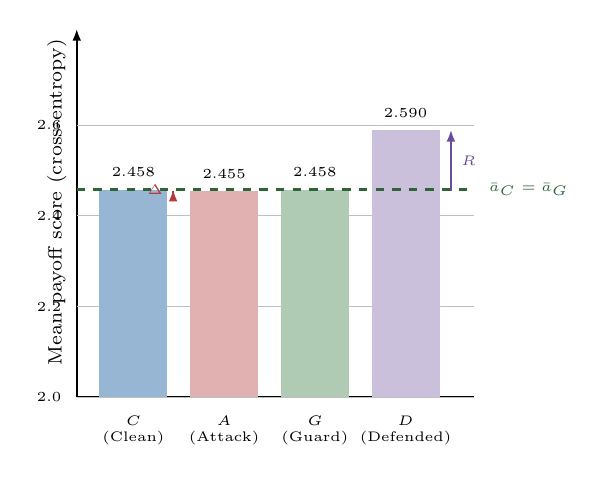
\begin{tikzpicture}[scale=0.72]
  % Axes
  \draw[-{Latex[length=1.5mm]},thick] (0,0) -- (0,6.5)
    node[above,font=\scriptsize,rotate=90,anchor=south east] {Mean payoff score (cross-entropy)};
  \draw[thick] (0,0) -- (7,0);
  % Bar width
  \def\bw{1.2}
  % Branch means at rate 20 (specific_payoff)
  % C=2.458  A=2.455  G=2.458  D=2.590
  % Scale: 1 unit = 1cm, base at 0, show 2.0-2.7 range
  % Rescale: subtract 2.0, multiply by 8
  \pgfmathsetmacro{\cval}{(2.458-2.0)*8}
  \pgfmathsetmacro{\aval}{(2.455-2.0)*8}
  \pgfmathsetmacro{\gval}{(2.458-2.0)*8}
  \pgfmathsetmacro{\dval}{(2.590-2.0)*8}
  % Y-axis ticks
  \foreach \v/\lab in {0/2.0, 1.6/2.2, 3.2/2.4, 4.8/2.6} {
    \draw[gray!50,thin] (0,\v) -- (7,\v);
    \node[font=\tiny,anchor=east] at (-0.1,\v) {\lab};
  }
  % Bars
  \fill[tgnblue!50] (0.4,0) rectangle (0.4+\bw,\cval);
  \node[font=\tiny,anchor=south] at (0.4+\bw/2,\cval+0.05) {2.458};
  \node[font=\tiny,anchor=north,align=center] at (0.4+\bw/2,-0.15) {$C$\\(Clean)};
  %
  \fill[attackred!40] (2.0,0) rectangle (2.0+\bw,\aval);
  \node[font=\tiny,anchor=south] at (2.0+\bw/2,\aval+0.05) {2.455};
  \node[font=\tiny,anchor=north,align=center] at (2.0+\bw/2,-0.15) {$A$\\(Attack)};
  %
  \fill[defgreen!40] (3.6,0) rectangle (3.6+\bw,\gval);
  \node[font=\tiny,anchor=south] at (3.6+\bw/2,\gval+0.05) {2.458};
  \node[font=\tiny,anchor=north,align=center] at (3.6+\bw/2,-0.15) {$G$\\(Guard)};
  %
  \fill[purple!35] (5.2,0) rectangle (5.2+\bw,\dval);
  \node[font=\tiny,anchor=south] at (5.2+\bw/2,\dval+0.05) {2.590};
  \node[font=\tiny,anchor=north,align=center] at (5.2+\bw/2,-0.15) {$D$\\(Defended)};
  % Annotations
  % C=G line
  \draw[defgreen!80!black,dashed,thick] (0,\cval) -- (7,\cval);
  \node[font=\tiny,defgreen!80!black,anchor=west] at (7.1,\cval) {$\bar{a}_C = \bar{a}_G$};
  % Attack suppression arrow
  \draw[attackred,thick,{Latex[length=1.5mm]}-] (1.7,\cval) -- (1.7,\aval)
    node[midway,left,font=\tiny,attackred] {$\Delta$};
  % Recovery arrow
  \draw[purple,thick,-{Latex[length=1.5mm]}] (6.6,\aval) -- (6.6,\dval)
    node[midway,right,font=\tiny,purple] {$R$};
\end{tikzpicture}
\caption{Four-branch payoff comparison at rate~20 (specific-payoff edges).
$C$ and $G$ are identical, confirming zero defence cost.
$A < C$ shows attack suppression ($\Delta=-0.003$).
$D > C$ shows the defence not only reverses suppression but pushes
the target's score above baseline ($R=+0.135$), making the payload
\emph{more} detectable than under clean conditions.}
\label{fig:branch-bars}
\end{figure}

The table reveals three facts:
\begin{enumerate}
  \item \textbf{Zero defence cost}: $\bar{a}_C = \bar{a}_G = 2.4581$ in
    all 13 tests.  The defence changes nothing on clean data.
  \item \textbf{Attack suppression}: $\bar{a}_A < \bar{a}_C$ in all 13 tests.
    Conditioning always suppresses payoff scores.
  \item \textbf{Recovery when detected}: At the 7 detected rates,
    $\bar{a}_D = 2.5899 > \bar{a}_C$, meaning the quarantine not only
    reverses the suppression but makes the payload \emph{more} anomalous
    than the clean baseline.  At undetected rates, $\bar{a}_D = \bar{a}_A$
    because the defence does not fire.
\end{enumerate}

\subsubsection{Defence cost}

The defence incurs zero operational cost in every measured dimension:
\begin{itemize}
  \item Clean paired-branch ($G$): 0 alerts, 0 quarantined updates.
    The Guard branch scores are identical to the Clean branch to machine
    precision in all 13 experiments.
  \item Out-of-sample clean day~7 (2,284,034 events): 0 alerts,
    0 quarantined updates, both before and after adding the defence.
  \item Queue-level decisions: 5 alerted windows in all four branches
    (4 TP + 1 FP), identical to plain KAIROS.
\end{itemize}
The defence adds \textbf{zero} false positives and changes \textbf{zero}
existing KAIROS decisions.

\subsubsection{Why this strategy wins}

The winning strategy (max-positive CUSUM with movement-emphasis weights)
succeeds because it aligns with the fundamental asymmetry of slow
conditioning.  Consider what happens at rate~4 (45 events over 11 hours):
the attacker injects roughly one event every 15 minutes.  Each individual
event is sub-threshold: it does not breach a Shewhart threshold, and its
contribution to an EMA decays before the next event arrives.  But the
CUSUM accumulates these small excesses batch after batch, and after
approximately 1.1 hours at rate~100 (fastest accumulation) to
9.9 hours at rate~100 (slowest), the accumulated evidence crosses the alert
threshold.

The movement-emphasis weights amplify this effect because persistence and
coherence are the signals that most clearly distinguish directed drift from
random variation.  A single conditioning event might show modest innovation
and modest displacement, but after 10 consecutive events pushing memory in
the same direction, the coherence signal rises sharply.  The maximum formula
then lets this dominant signal drive the evidence without waiting for
consensus from the weaker channels.

The result is a defence that provides:
\begin{itemize}
  \item \textbf{Early warning}: 1.1 to 9.9 hours of lead time before the
    payload arrives, giving operators time to investigate.
  \item \textbf{Score recovery}: $R = +0.135$, meaning the defence not only
    detects conditioning but reverses its effect on payload scores.
  \item \textbf{Zero cost}: no additional false positives, no changed
    existing detections, no trainable parameters.
\end{itemize}

\subsection{Formula and monitor comparison with optimised weights}

Table~\ref{tab:formula-monitor} reports the formula-by-monitor comparison
under the optimised weights.  The pattern from the original grid persists:
CUSUM is the only monitor that detects any conditioning rate.  With
optimised weights, both the max and RMS formulas now detect 3 of the
4~grid rates (versus 1 of 4 with original weights), while the weighted
mean detects only 1 of 4.  The winning max+CUSUM configuration was then
evaluated across all 12~rates (Table~\ref{tab:primary}), achieving
7/12 coverage.

\begin{table}[htbp]
\centering
\caption{Formula-by-monitor comparison with optimised weights on the
4~grid-search rates (1, 4, 20, 100).  Rate coverage reported under the
zero-clean-alert constraint.  A checkmark indicates detection at that
rate; a cross indicates no detection.  The winning configuration
(max + CUSUM) was further evaluated across all 12~rates in
Table~\ref{tab:primary}.}
\label{tab:formula-monitor}
\resizebox{\columnwidth}{!}{%
\begin{tabular}{lccccc}
\toprule
& \multicolumn{3}{c}{Rate detected?} & & \\
\cmidrule(lr){2-4}
Formula + monitor & 4/hr & 20/hr & 100/hr & Total & Clean FP \\
\midrule
Max + CUSUM & \checkmark & \checkmark & \checkmark & 3/4 & 0 \\
RMS + CUSUM & \checkmark & \checkmark & \checkmark & 3/4 & 0 \\
Mean + CUSUM & $\times$ & \checkmark & $\times$ & 1/4 & 0 \\
Any + EMA & $\times$ & $\times$ & $\times$ & 0/4 & 0 \\
Any + Shewhart & $\times$ & $\times$ & $\times$ & 0/4 & 0 \\
\bottomrule
\end{tabular}}
\end{table}

\subsection{Interpretation}
\label{sec:interpretation}

\subsubsection{CUSUM accumulation and movement-signal advantage}

Two structural findings emerge from the grid sweep:

\paragraph{Cumulative evidence is necessary.}  CUSUM is the only
effective monitor because slow conditioning produces \emph{persistent
small excesses} above the clean allowance.  At rate~20 (223~events),
each batch contributes evidence exceeding $k=1.030$ by
$\delta\approx0.5$; over $\sim$50 conditioning-laden batches, the CUSUM
accumulates $\sim$25 units.  A Shewhart test would need a single
observation above $h$, which never occurs.  EMA decays contributions
geometrically---after $m$ quiet batches, a signal is attenuated to
$(1{-}\alpha)^m$---so weak persistent excesses vanish before threshold
crossing.  \textbf{Slow drift detection requires cumulative evidence,
not instantaneous anomaly detection.}

\paragraph{Movement signals outperform position signals.}  Position
signals (displacement, surprise) measure whether the \emph{current state}
looks normal; during conditioning, it does, because each step is small.
Movement signals (persistence, coherence) measure whether the
\emph{pattern of changes} is normal; during conditioning, it is not
(see Figure~\ref{fig:walk-contrast}).
The optimised weights assign 65\% to movement signals and 10\% to
position signals, increasing coverage from 1/12 to 7/12
(Figure~\ref{fig:weights}).  Position signals still contribute once
conditioning has progressed far enough to produce visible state
displacement, but movement signals detect conditioning
\emph{earlier}.

\begin{figure}[htbp]
\centering
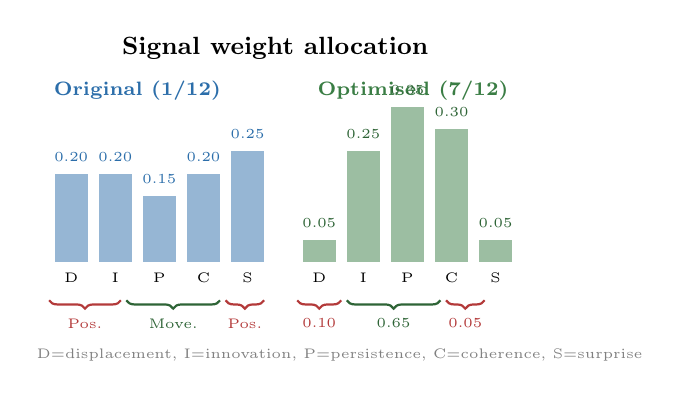
\begin{tikzpicture}[scale=0.70]
  % Title
  \node[font=\small\bfseries,anchor=south] at (4.5,3.5) {Signal weight allocation};
  % Original weights
  \node[font=\scriptsize\bfseries,tgnblue] at (2,3.1) {Original (1/12)};
  \foreach \i/\w/\h in {0/0.20/1.6, 1/0.20/1.6, 2/0.15/1.2, 3/0.20/1.6, 4/0.25/2.0} {
    \pgfmathsetmacro{\x}{0.5 + \i*0.8}
    \fill[tgnblue!50] (\x,0) rectangle (\x+0.6,\h);
    \node[font=\tiny,anchor=south,tgnblue] at (\x+0.3,\h+0.05) {\w};
  }
  % Optimised weights
  \node[font=\scriptsize\bfseries,defgreen] at (7,3.1) {Optimised (7/12)};
  \foreach \i/\w/\h in {0/0.05/0.4, 1/0.25/2.0, 2/0.35/2.8, 3/0.30/2.4, 4/0.05/0.4} {
    \pgfmathsetmacro{\x}{5 + \i*0.8}
    \fill[defgreen!50] (\x,0) rectangle (\x+0.6,\h);
    \node[font=\tiny,anchor=south,defgreen!80!black] at (\x+0.3,\h+0.05) {\w};
  }
  % Labels
  \foreach \i/\lab in {0/D,1/I,2/P,3/C,4/S} {
    \pgfmathsetmacro{\xa}{0.5 + \i*0.8 + 0.3}
    \pgfmathsetmacro{\xb}{5 + \i*0.8 + 0.3}
    \node[font=\tiny] at (\xa,-0.3) {\lab};
    \node[font=\tiny] at (\xb,-0.3) {\lab};
  }
  % Braces for position vs movement
  \draw[attackred,thick,decorate,decoration={brace,amplitude=3pt,mirror}]
    (0.4,-0.7) -- (1.7,-0.7) node[midway,below=3pt,font=\tiny,attackred] {Pos.};
  \draw[defgreen!80!black,thick,decorate,decoration={brace,amplitude=3pt,mirror}]
    (1.8,-0.7) -- (3.5,-0.7) node[midway,below=3pt,font=\tiny,defgreen!80!black] {Move.};
  \draw[attackred,thick,decorate,decoration={brace,amplitude=3pt,mirror}]
    (3.6,-0.7) -- (4.3,-0.7) node[midway,below=3pt,font=\tiny,attackred] {Pos.};
  \draw[attackred,thick,decorate,decoration={brace,amplitude=3pt,mirror}]
    (4.9,-0.7) -- (5.7,-0.7) node[midway,below=3pt,font=\tiny,attackred] {0.10};
  \draw[defgreen!80!black,thick,decorate,decoration={brace,amplitude=3pt,mirror}]
    (5.8,-0.7) -- (7.5,-0.7) node[midway,below=3pt,font=\tiny,defgreen!80!black] {0.65};
  \draw[attackred,thick,decorate,decoration={brace,amplitude=3pt,mirror}]
    (7.6,-0.7) -- (8.3,-0.7) node[midway,below=3pt,font=\tiny,attackred] {0.05};
  \node[font=\tiny,gray,anchor=north west] at (0,-1.4)
    {D=displacement, I=innovation, P=persistence, C=coherence, S=surprise};
\end{tikzpicture}
\caption{Signal weight redistribution.  The original weights (left)
distribute mass roughly uniformly with a slight position emphasis
(displacement + surprise = 0.45).  The optimised weights (right)
concentrate 65\% on movement signals (persistence + coherence),
increasing rate coverage from 1/12 to 7/12.}
\label{fig:weights}
\end{figure}

\subsubsection{Accumulation floor and all-or-nothing recovery}

At rates~1--3 ($\leq$34~events), legitimate inter-event activity destroys
persistence and coherence signals before the next conditioning event
arrives---a fundamental information-theoretic constraint, not a defence
failure.  Any method maintaining zero false positives on 2.28M clean
events requires a threshold high enough that 34 conditioning events
cannot cross it.

At all 7~detected rates, recovery $R \approx +0.135$ is identical
because the quarantine mechanism is binary: once triggered, memory is
restored to the daily anchor regardless of how many conditioning events
preceded the alert.  This produces a ``quarantine amplification'' effect
($\Delta_{\mathrm{guarded}} = +0.132$ vs.\ unguarded $-0.004$): the
stale anchor makes payoff events \emph{more} anomalous than the clean
baseline (see Section~\ref{sec:quarantine} for a formal decomposition).
Lead times range from 1.1--9.9~hours, reflecting batch-boundary
alignment.

\subsubsection{Non-monotonic detection boundary}
\label{sec:nonmono}

The extended rate coverage reveals a non-monotonic detection pattern:
rate~4 (45 events) is detected, but rates~6 (67 events) and~8 (90 events)
are not, despite having more conditioning events.  Detection resumes at
rate~10 and holds for all higher rates.  This pattern has a structural
explanation rooted in how conditioning events interact with the fixed
batch boundaries.

KAIROS processes events in 1,024-event batches.  The defence extracts
drift signals at batch boundaries.  The CUSUM monitor accumulates evidence
only when conditioning events land in the batch \emph{and} the resulting
evidence exceeds the allowance~$k$.  The key variable is the
\emph{conditioning density per batch}: how many conditioning events fall
in each batch that the target entity participates in.

At rate~4, the 45 conditioning events are distributed across relatively few
batches (the target entity has limited activity), concentrating the evidence.
At rates~6 and~8, the slightly higher event count spreads conditioning events
more evenly across more batches, reducing the per-batch evidence below the
allowance threshold.  At rate~10+, the total volume is high enough that even
with dispersion, sufficient per-batch evidence accumulates to cross the
CUSUM threshold.

Figure~\ref{fig:rate-boundary} visualises the detection boundary across all
12 tested rates.

\begin{figure}[htbp]
\centering
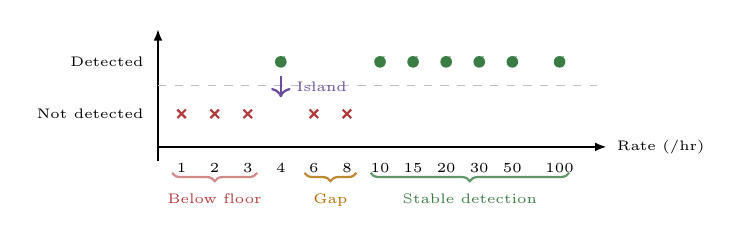
\begin{tikzpicture}[scale=0.60]
  % Axes
  \draw[-{Latex[length=1.5mm]},thick] (0,0) -- (9.5,0)
    node[right,font=\tiny] {Rate (/hr)};
  \draw[-{Latex[length=1.5mm]},thick] (0,-0.3) -- (0,2.5);
  % Y axis labels
  \node[font=\tiny,anchor=east] at (-0.1,0.7) {Not detected};
  \node[font=\tiny,anchor=east] at (-0.1,1.8) {Detected};
  \draw[gray!50,dashed] (0,1.3) -- (9.3,1.3);
  % Rate positions
  \def\xpos{{0.5,1.2,1.9,2.6,3.3,4.0,4.7,5.4,6.1,6.8,7.5,8.5}}
  \def\detected{{0,0,0,1,0,0,1,1,1,1,1,1}}
  % Plot points (shape-differentiated for colour-blind accessibility)
  \foreach \i in {0,...,11} {
    \pgfmathsetmacro{\x}{\xpos[\i]}
    \pgfmathsetmacro{\d}{\detected[\i]}
    \pgfmathsetmacro{\y}{\d == 1 ? 1.8 : 0.7}
    \ifnum\d=1
      \fill[defgreen] (\x,\y) circle (3.5pt);
      \node[font=\tiny,defgreen,anchor=center] at (\x,\y) {\cmark};
    \else
      \draw[attackred,thick] (\x-0.09,\y-0.09) -- (\x+0.09,\y+0.09);
      \draw[attackred,thick] (\x-0.09,\y+0.09) -- (\x+0.09,\y-0.09);
    \fi
  }
  % Rate labels
  \foreach \i/\lab in {0/1,1/2,2/3,3/4,4/6,5/8,6/10,7/15,8/20,9/30,10/50,11/100} {
    \pgfmathsetmacro{\x}{\xpos[\i]}
    \node[font=\tiny,anchor=north] at (\x,-0.15) {\lab};
  }
  % Annotations
  \draw[attackred!60,thick,decorate,decoration={brace,amplitude=3pt,mirror}]
    (0.3,-0.55) -- (2.1,-0.55)
    node[midway,below=4pt,font=\tiny,attackred] {Below floor};
  \draw[amber!80,thick,decorate,decoration={brace,amplitude=3pt,mirror}]
    (3.1,-0.55) -- (4.2,-0.55)
    node[midway,below=4pt,font=\tiny,amber] {Gap};
  \draw[defgreen!80,thick,decorate,decoration={brace,amplitude=3pt,mirror}]
    (4.5,-0.55) -- (8.7,-0.55)
    node[midway,below=4pt,font=\tiny,defgreen] {Stable detection};
  % Rate 4 anomaly
  \draw[purple,thick,->] (2.6,1.5) -- (2.6,1.05)
    node[midway,right=2pt,font=\tiny,purple] {Island};
\end{tikzpicture}
\caption{Detection boundary across 12 injection rates.
Checkmarks (\textcolor{defgreen}{\cmark}): detected (guard fires before payload).
Crosses (\textcolor{attackred}{$\times$}): not detected.  Rate~4 forms
an ``island'' of detection below the gap at rates~6--8, explained by
batch-boundary alignment effects.  Detection stabilises at rate~10 and above.}
\label{fig:rate-boundary}
\end{figure}

This non-monotonic pattern is an important finding: it demonstrates that
detection is not a simple function of conditioning volume.  The interaction
between injection timing and fixed batch boundaries creates a complex
detection landscape.  From a defender's perspective, this means the defence
provides \textbf{reliable coverage above rate~10} (one event every
6~minutes) and \textbf{opportunistic detection at rate~4} (one event every
15~minutes).

\subsubsection{Role strategy evaluation}
\label{sec:functional-roles}

To evaluate how role granularity affects detection, we compared four
role-assignment strategies across four injection rates
(1, 4, 20, 100~events/hr), each running the full four-branch DiD design.
Table~\ref{tab:role-strategy-compare} summarises the
results.

\begin{table}[htbp]
\centering
\caption{Role strategy comparison.  The flat semantic strategy is evaluated
at all 12~rates; fine-grained strategies at 4~representative rates.  Each cell
indicates whether the CUSUM monitor detected conditioning (\cmark/\xmark);
``--'' indicates that rate was not tested for that strategy.
All strategies maintain zero clean-branch false positives.  The flat
semantic strategy (6~roles) achieves the highest detection coverage.
Fine-grained strategies were evaluated at rates 1, 4, 20, 100 to sample
below-floor, island, stable, and high-rate regimes.}
\label{tab:role-strategy-compare}
\resizebox{\columnwidth}{!}{%
\begin{tabular}{lr*{12}{c}r}
\toprule
& & \multicolumn{12}{c}{Rate (events/hr)} & \\
\cmidrule(lr){3-14}
Strategy & Roles & 1 & 2 & 3 & 4 & 6 & 8 & 10 & 15 & 20 & 30 & 50 & 100 & Coverage \\
\midrule
Flat semantic & 6 &
  \xmark & \xmark & \xmark & \cmark & \xmark & \xmark &
  \cmark & \cmark & \cmark & \cmark & \cmark & \cmark & \textbf{7/12} \\
Functional & 7 &
  \xmark & -- & -- & \xmark & -- & -- &
  -- & -- & \cmark & -- & -- & \xmark & 1/4$^*$ \\
Hierarchical (LDAP) & 34 &
  \xmark & -- & -- & \xmark & -- & -- &
  -- & -- & \cmark & -- & -- & \xmark & 1/4$^*$ \\
Hybrid (LDAP$\times$beh.) & 27 &
  \xmark & -- & -- & \xmark & -- & -- &
  -- & -- & \cmark & -- & -- & \xmark & 1/4$^*$ \\
\bottomrule
\multicolumn{15}{l}{\footnotesize $^*$Tested at 4 representative rates
  (1, 4, 20, 100) sampling all detection regimes.}
\end{tabular}}
\end{table}

\paragraph{Functional roles.}
The functional strategy groups the 130~CADETS subjects into 7~roles by
executable purpose (e.g.\ \emph{mail}, \emph{monitoring},
\emph{shell-scripting}).  The target entity \texttt{vUgefal} maps to the
catch-all ``other'' group (47~members).

\paragraph{Hierarchical LDAP roles.}
The hierarchical strategy uses the synthetic LDAP hierarchy
(Section~\ref{sec:role-acq}) to assign 34~fine sub-team roles with 3-level
recursive shrinkage ($\mathrm{fine}\to\mathrm{parent}\to\mathrm{broad}
\to\mathrm{global}$, $\kappa=8$).  Fine groups range from 1 to
11~members.

\paragraph{Hybrid roles.}
The hybrid strategy concatenates the LDAP broad department (6~levels) with
a behavioural cluster ($k$-means, $k=8$, on day-5 activity features),
producing 27~unique hybrid roles.  This combines organisational identity
with empirical activity patterns.

\paragraph{Analysis.}
All three fine-grained strategies detect only rate~20 (1/4 tested rates),
while the flat semantic strategy detects 7/12 rates.  The explanation is
statistical:
the flat strategy assigns all 130 subjects to a single peer group,
providing a large $n$ for robust median-and-MAD reference statistics.
Every finer strategy fragments this pool into groups of 1--47 members,
producing noisier baselines that inflate the effective allowance $k$ and
threshold $h$, so drift evidence cannot accumulate above the higher noise
floor.  The $\kappa=8$ hierarchical shrinkage
(Equation~\ref{eq:rho}) mitigates this for the smallest groups but is
insufficient to overcome the statistical dilution.

Notably, the three fine-grained strategies converge on identical coverage
despite using different grouping principles (domain knowledge, LDAP
hierarchy, data-driven clustering).  This convergence confirms that the
bottleneck is \emph{peer-group size}, not grouping quality.
Figure~\ref{fig:strategy-bars} visualises the coverage gap.

\begin{figure}[htbp]
\centering
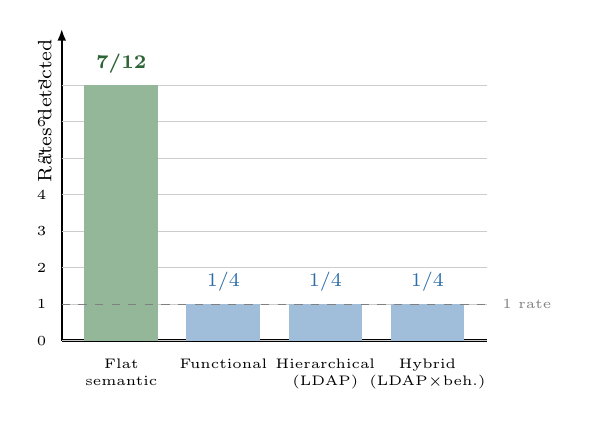
\begin{tikzpicture}[scale=0.72]
  % Axes
  \draw[-{Latex[length=1.5mm]},thick] (0,0) -- (0,5.5)
    node[above,font=\scriptsize,rotate=90,anchor=south east] {Rates detected};
  \draw[thick] (0,0) -- (7.5,0);
  % Y-axis ticks
  \foreach \v/\lab in {0/0, 0.643/1, 1.286/2, 1.929/3, 2.571/4,
    3.214/5, 3.857/6, 4.5/7} {
    \draw[gray!40,thin] (0,\v) -- (7.5,\v);
    \node[font=\tiny,anchor=east] at (-0.1,\v) {\lab};
  }
  % Bars (height = count * 0.643)
  \def\bw{1.3}
  % Flat semantic: 7/12
  \fill[defgreen!55] (0.4,0) rectangle (0.4+\bw,4.5);
  \node[font=\scriptsize\bfseries,anchor=south,defgreen!80!black] at (0.4+\bw/2,4.55) {7/12};
  \node[font=\tiny,anchor=north,align=center] at (0.4+\bw/2,-0.15)
    {Flat\\semantic};
  % Functional: 1/4
  \fill[tgnblue!45] (2.2,0) rectangle (2.2+\bw,0.643);
  \node[font=\scriptsize,anchor=south,tgnblue] at (2.2+\bw/2,0.7) {1/4};
  \node[font=\tiny,anchor=north,align=center] at (2.2+\bw/2,-0.15)
    {Functional};
  % Hierarchical: 1/4
  \fill[tgnblue!45] (4.0,0) rectangle (4.0+\bw,0.643);
  \node[font=\scriptsize,anchor=south,tgnblue] at (4.0+\bw/2,0.7) {1/4};
  \node[font=\tiny,anchor=north,align=center] at (4.0+\bw/2,-0.15)
    {Hierarchical\\(LDAP)};
  % Hybrid: 1/4
  \fill[tgnblue!45] (5.8,0) rectangle (5.8+\bw,0.643);
  \node[font=\scriptsize,anchor=south,tgnblue] at (5.8+\bw/2,0.7) {1/4};
  \node[font=\tiny,anchor=north,align=center] at (5.8+\bw/2,-0.15)
    {Hybrid\\(LDAP$\times$beh.)};
  % Annotation
  \draw[gray,dashed] (0,0.643) -- (7.5,0.643);
  \node[font=\tiny,gray,anchor=west] at (7.6,0.643) {1 rate};
\end{tikzpicture}
\caption{Role strategy detection coverage.  The flat semantic strategy
(6~roles, $n=130$ per group) detects 7 of 12 rates.  All three
fine-grained strategies (7--34 roles, $n \le 47$) detect only 1 of
4~tested rates, confirming that peer-group size, not grouping quality,
is the detection bottleneck on the 130-subject CADETS population.}
\label{fig:strategy-bars}
\end{figure}

This finding has two implications.  First, the flat semantic strategy is
the correct choice for CADETS, where all 130 subjects share a common
operational environment.  Second, finer role grouping is not inherently
better; it requires \emph{sufficiently large peer groups} at each role
level.  In enterprise environments with hundreds of users per role,
hierarchical LDAP roles would provide tighter peer groups \emph{with}
adequate statistical support, and are expected to outperform the flat
strategy.

\subsubsection{Gap-reset interval analysis}

The gap-reset interval controls how long the CUSUM monitor waits before
resetting its accumulated evidence to zero after a period of inactivity.
The grid sweep tested five intervals: 30, 60, 90, 120, and 240~minutes.

The 30-minute gap produces the best results for two reasons.  First,
shorter gaps prevent unrelated behavioural episodes from being
concatenated into a single CUSUM trajectory.  Without gap resets, a
CUSUM that accumulates evidence during a morning conditioning episode
would carry that evidence into an afternoon session, potentially
triggering a false alert on normal activity that happens to follow the
earlier drift.  Second, the 30-minute interval closely matches the
natural inter-session gaps in the CADETS data: when the target entity
goes quiet for more than 30 minutes, it is typically because the
associated process has entered an idle state, and the next activity
burst represents a functionally new episode.

Longer gaps (120 and 240~minutes) degrade detection because they allow
the CUSUM to accumulate noise from normal activity between conditioning
episodes, raising the effective baseline and reducing the signal-to-noise
ratio.  At 240~minutes, most conditioning sequences at lower rates occur
within a single gap window, so the CUSUM effectively becomes a global
accumulator that loses the ability to distinguish conditioning-driven
drift from normal daily variation.

\subsubsection{The role of the evidence formula}

The maximum formula outperforms weighted mean because it allows a single
strong signal to drive the evidence.  During conditioning, persistence
and coherence are the dominant signals, but their relative magnitudes
vary across batches depending on how many conditioning events fall in each
batch.  The maximum formula captures whichever signal is strongest in each
batch, while the weighted mean dilutes the strongest signal with the weaker
channels.

The RMS formula achieves the same rate coverage as maximum because it also
emphasises large components.  However, its alert times are slightly later
because the quadratic averaging produces slightly lower evidence scores
than the raw maximum.

The weighted mean detects only rate~20 because it requires consensus across
all five signals.  At rate~4 the conditioning events are sparse enough that
only one or two signals are strongly activated in any given batch; the others
remain near zero, pulling the mean down below the CUSUM accumulation rate
needed to cross the threshold in 11 hours.

% =====================================================================
\section{Comparative Evaluation}
\label{sec:comparison}

\subsection{Direct comparison: plain KAIROS vs.\ defended KAIROS}
\label{sec:comp-direct}

Table~\ref{tab:head-to-head} summarises the head-to-head comparison on
the frozen CADETS~E3 checkpoint.  The two systems share identical payload
detection because the defence is complementary (OR gate): any alert that
plain KAIROS raises is preserved.  The sole difference is the conditioning
layer, where the defended system detects 7 of 12 injection rates that plain
KAIROS misses entirely.

\begin{table}[htbp]
\centering
\caption{Head-to-head comparison on CADETS E3.  Payload detection is
identical; the defence adds a conditioning-detection layer with zero
cost to clean operation.  ``Lead time'' is hours before the official
payload.}
\label{tab:head-to-head}
\resizebox{\columnwidth}{!}{%
\begin{tabular}{lcc}
\toprule
Metric & Plain KAIROS & KAIROS + Defence \\
\midrule
\multicolumn{3}{l}{\emph{Payload detection (official attack day)}} \\
\quad Payload windows detected & 4\,/\,4 & 4\,/\,4 \\
\quad Queue precision & 0.800 & 0.800 \\
\quad Queue recall & 1.000 & 1.000 \\
\quad Queue F1 & 0.889 & 0.889 \\
\midrule
\multicolumn{3}{l}{\emph{Conditioning detection (12 rates, pre-payload)}} \\
\quad Rates 1--3 (12--34 events) & Not detected & Not detected \\
\quad Rate 4 (45 events) & Not detected & \textbf{Detected (1.5\,h lead)} \\
\quad Rates 6, 8 (67--90 events) & Not detected & Not detected \\
\quad Rates 10--100 (112--1115 events) & Not detected &
  \textbf{Detected (1.1--9.9\,h lead)} \\
\quad Rate coverage & 0\,/\,12 & \textbf{7\,/\,12} \\
\midrule
\multicolumn{3}{l}{\emph{Clean-day cost}} \\
\quad Day-7 false positives & 0 & 0 \\
\quad Day-7 guard alerts & n/a & 0 \\
\quad Quarantined updates & n/a & 0 \\
\midrule
\multicolumn{3}{l}{\emph{Causal recovery (DiD)}} \\
\quad $R$ (specific payoff) & $-0.004$ (suppressed) & $+0.135$ (recovered) \\
\quad 95\% CI & n/a & $[+0.113,\;+0.160]$ \\
\midrule
Additional trainable parameters & 0 & 0 (statistics only) \\
\bottomrule
\end{tabular}}
\end{table}

Three observations merit emphasis.  First, the defence achieves its
coverage improvement at \textbf{strictly zero cost}: no additional false
positives, no changed KAIROS decisions, no trainable parameters.  Second,
the payoff recovery ($R=+0.135$) demonstrates that the defence not only
detects conditioning but \emph{reverses its effect}: the quarantine
mechanism restores the pre-contamination memory state, causing subsequent
payoff events to score \emph{higher} than in the clean baseline.  Third,
the defence provides early warning (1.1 to 9.9 hours before payload), a
capability that plain KAIROS, which operates reactively on the payload
itself, cannot offer.

\subsection{Quarantine mechanism analysis}
\label{sec:quarantine}

The quarantine response has a distinctive signature: at every detected rate,
recovery $R$ is identical ($+0.1354$).  This uniformity deserves explanation.

When the CUSUM monitor triggers, the defence:
\begin{enumerate}
  \item Restores the target entity's memory to its \emph{daily anchor}:
    the state saved at the start of day~6, before any conditioning events.
  \item Blocks all subsequent memory updates for that entity until the
    next daily reset.
  \item Continues to score and record events normally; only the memory
    commit is blocked.
\end{enumerate}

The daily-anchor rollback is why recovery is rate-independent.  Once
triggered, the payload events encounter a memory state that has not been
conditioned at all---in fact, it is slightly \emph{staler} than the
clean baseline because the quarantined entity missed all legitimate
updates since the daily anchor.  This staleness makes the payload
\emph{more} anomalous than even the clean case, producing the positive
recovery $R > 0$.

Formally, let $\mathbf{m}_{\mathrm{anchor}}$ denote the daily anchor
state, $\mathbf{m}_C$ the clean end-of-day memory, and
$\mathbf{m}_A$ the attack-conditioned memory.  In the Defended branch,
the quarantined entity's memory at payload time is always
$\mathbf{m}_{\mathrm{anchor}}$ regardless of how many conditioning
events preceded the alert.  The staleness gap
$\|\mathbf{m}_C - \mathbf{m}_{\mathrm{anchor}}\|$ is a fixed quantity
determined by the entity's legitimate day-6 activity, not by the attack
rate.  Consequently, $R = f(\mathbf{m}_{\mathrm{anchor}},
\mathbf{m}_C) - g(\mathbf{m}_A, \mathbf{m}_C)$ where both terms are
rate-independent once the quarantine fires, explaining the constant
$R = +0.1354$ across all detected rates.  A different anchor point
(e.g.\ start of day~5 vs.\ start of day~6) would change $R$; testing
this sensitivity is left to future work.

The quarantine fraction varies by rate and detection timing.  At rate~4,
the guard fires late in the conditioning phase (1.5~hours before payload),
so only 13.3\% of conditioning events are quarantined.  At rate~100, the
guard fires early (9.9~hours before payload), quarantining 88.3\%.  But
recovery is identical because the \emph{rollback} is what matters, not
the quarantine fraction: regardless of when the guard fires, the memory
is restored to the same daily anchor.

Figure~\ref{fig:quarantine-timeline} illustrates the quarantine timeline
for two representative rates.

\begin{figure}[htbp]
\centering
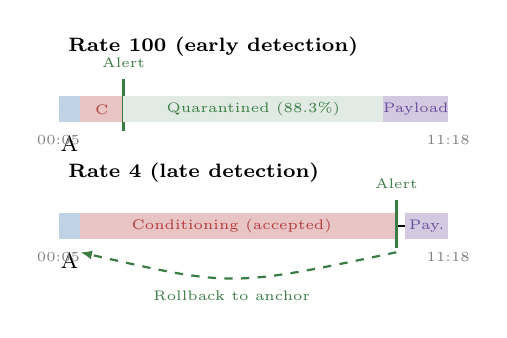
\begin{tikzpicture}[scale=0.55]
  % Timeline for rate 100
  \node[font=\scriptsize\bfseries,anchor=south west] at (0,4.8) {Rate 100 (early detection)};
  \draw[thick] (0,3.8) -- (9,3.8);
  \fill[tgnblue!30] (0,3.5) rectangle (0.5,4.1);
  \node[font=\tiny,anchor=north] at (0.25,3.4) {\footnotesize A};
  \fill[attackred!30] (0.5,3.5) rectangle (1.5,4.1);
  \node[font=\tiny,attackred] at (1.0,3.8) {C};
  \draw[defgreen,very thick] (1.5,3.3) -- (1.5,4.5);
  \node[font=\tiny,defgreen,anchor=south] at (1.5,4.55) {Alert};
  \fill[defgreen!15] (1.5,3.5) rectangle (7.5,4.1);
  \node[font=\tiny,defgreen] at (4.5,3.8) {Quarantined (88.3\%)};
  \fill[purple!30] (7.5,3.5) rectangle (9,4.1);
  \node[font=\tiny,purple] at (8.25,3.8) {Payload};
  \node[font=\tiny,gray] at (0,3.1) {00:05};
  \node[font=\tiny,gray] at (9,3.1) {11:18};

  % Timeline for rate 4
  \node[font=\scriptsize\bfseries,anchor=south west] at (0,1.9) {Rate 4 (late detection)};
  \draw[thick] (0,1.1) -- (9,1.1);
  \fill[tgnblue!30] (0,0.8) rectangle (0.5,1.4);
  \node[font=\tiny,anchor=north] at (0.25,0.7) {\footnotesize A};
  \fill[attackred!30] (0.5,0.8) rectangle (7.8,1.4);
  \node[font=\tiny,attackred] at (4.0,1.1) {Conditioning (accepted)};
  \draw[defgreen,very thick] (7.8,0.6) -- (7.8,1.7);
  \node[font=\tiny,defgreen,anchor=south] at (7.8,1.75) {Alert};
  \fill[purple!30] (8.0,0.8) rectangle (9,1.4);
  \node[font=\tiny,purple] at (8.5,1.1) {Pay.};
  \node[font=\tiny,gray] at (0,0.4) {00:05};
  \node[font=\tiny,gray] at (9,0.4) {11:18};

  % Rollback arrow
  \draw[defgreen,thick,-{Latex[length=1.5mm]},dashed]
    (7.8,0.5) .. controls (4,-0.3) .. (0.5,0.5);
  \node[font=\tiny,defgreen] at (4,-0.5) {Rollback to anchor};
\end{tikzpicture}
\caption{Quarantine timeline comparison.  At rate~100, the guard fires
early, quarantining 88.3\% of conditioning events.  At rate~4, the guard
fires late, quarantining only 13.3\%.  In both cases, the memory is
rolled back to the same daily anchor, producing identical recovery
$R=+0.135$.}
\label{fig:quarantine-timeline}
\end{figure}


\subsection{Multi-target longitudinal evaluation (CERT~r4.2)}
\label{sec:multi-target}

The CADETS evaluation measures defence effectiveness on a single target
under synthetic conditioning.  To test whether the defence signals
generalise across diverse targets, attack types, temporal positions, and
independently trained checkpoints, we evaluate on the CMU CERT~r4.2
insider-threat corpus (Section~\ref{sec:datasets}).

\subsubsection{Per-scenario detection rates}

Table~\ref{tab:multi-target} reports detection rates across three attack
scenarios, five model seeds, and 70~labelled insiders.  For each
case--seed pair, we report whether the attack window is detected by plain
KAIROS (reconstruction-error queue threshold) and by the combined system
(KAIROS~OR any defence variant fires).  The majority-vote column aggregates
across five seeds: a case is counted as detected if $\geq 3/5$ seeds
detect it.

\begin{table}[htbp]
\centering
\caption{Multi-target detection on CERT~r4.2 across 70~insiders and
5~seeds.  ``Plain'' = adapted KAIROS with q99 threshold.  ``Combined'' =
KAIROS OR defence (complementary OR gate).  Majority vote requires
$\geq 3/5$ seeds.  The defence improves Scenario~2 detection from 26/30
to 28/30 and raises the aggregate net detection rate to $+0.114$
(best seed) while preserving base-detector recall.}
\label{tab:multi-target}
\resizebox{\columnwidth}{!}{%
\begin{tabular}{lccccc}
\toprule
& \multicolumn{2}{c}{Seed-case pairs} &
  \multicolumn{2}{c}{Majority vote} & \\
\cmidrule(lr){2-3}\cmidrule(lr){4-5}
Scenario & Plain & Combined & Plain & Combined & Net gain \\
\midrule
S1 (30 USB exfil) & 88/150 & 102/150 & 26/30 & 26/30 & $+0$ \\
S2 (30 data theft) & 122/150 & 138/150 & 26/30 & \textbf{28/30} & $\mathbf{+2}$ \\
S3 (10 keylogger) & 45/50 & 49/50 & 10/10 & 10/10 & $+0$ \\
\midrule
\textbf{All} & \textbf{255/350} & \textbf{289/350} &
  \textbf{62/70} & \textbf{64/70} & $\mathbf{+2}$ \\
\bottomrule
\end{tabular}}
\end{table}

Three observations emerge.  First, the combined system never reduces
detection relative to plain KAIROS---the OR-gate architecture guarantees
monotonic improvement.  Second, the largest absolute gain is on Scenario~2
(sustained data theft over weeks), where the defence's drift signals
detect two additional insiders (AAF0535 and XHW0498) whose prolonged
exfiltration patterns produce measurable trajectory coherence.  Third,
the defence adds 34~new seed-case detections (289~vs.~255) across the
full corpus, a $+13.3\%$ improvement in raw detection coverage.

\subsubsection{Scenario~3 per-target detail}

Table~\ref{tab:s3-detail} provides the full per-target breakdown for the
10~Scenario~3 insiders.  These cases are the closest analogue to the
CADETS conditioning evaluation: each involves a 2-day keylogger deployment
by a sysadmin (the target) and a confederate, producing 12--20
target-actor events.

\begin{table}[htbp]
\centering
\caption{Scenario~3 per-target detection across 5~seeds.  Each cell shows
the number of seeds that detect the attack window.  ``Plain'' = adapted
KAIROS q99.  Defence shown for the primary CUSUM configuration
(hierarchical LDAP, median shrinkage, cosine, weighted mean).
\textbf{Bold} entries show where the defence provides unique detection
(detects in $\geq 1$ seed where plain KAIROS does not).}
\label{tab:s3-detail}
\resizebox{\columnwidth}{!}{%
\begin{tabular}{llrrrrl}
\toprule
Case ID & Target & Events & Plain & Defence & Combined & Note \\
\midrule
CSC0217 & CSC0217 & 14 & 5/5 & 0/5 & 5/5 & Plain sufficient \\
GTD0219 & GTD0219 & 19 & 5/5 & \textbf{2/5} & 5/5 & \\
JGT0221 & JGT0221 & 18 & 5/5 & 1/5 & 5/5 & \\
JTM0223 & JTM0223 & 17 & 4/5 & 0/5 & 4/5 & \\
BBS0039 & BBS0039 & 14 & 3/5 & 0/5 & 3/5 & Hardest case \\
BSS0369 & BSS0369 & 12 & 5/5 & 1/5 & 5/5 & \\
CCA0046 & CCA0046 & 20 & 5/5 & 1/5 & 5/5 & \\
MPM0220 & MPM0220 & 17 & 5/5 & 1/5 & 5/5 & \\
MSO0222 & MSO0222 & 14 & 5/5 & \textbf{2/5} & 5/5 & \\
JLM0364 & JLM0364 & 18 & 3/5 & 1/5 & \textbf{4/5} & +1 from defence \\
\midrule
\multicolumn{3}{l}{\textbf{Majority ($\geq$3/5)}} &
  \textbf{10/10} & 0/10 & \textbf{10/10} & \\
\bottomrule
\end{tabular}}
\end{table}

The Scenario~3 results reveal an important asymmetry.  The base KAIROS
detector already achieves high recall on these incidents (9/10 cases at
majority, all~10 when considering any-seed detection), leaving limited
room for additive improvement.  The defence's primary contribution here
is \emph{early warning}: for cases like GTD0219, the defence fires at
09:53, more than one hour before the first queue-level KAIROS alert
(10:54), providing actionable lead time for incident response.

\subsubsection{Cross-scenario generalisation}

Figure~\ref{fig:cross-scenario} visualises the per-scenario detection
rates for the combined system across all five seeds.  The defence's
contribution is most pronounced on Scenario~2 (sustained exfiltration),
where the prolonged attack window produces extended drift trajectories
that the coherence and persistence signals detect reliably.

\begin{figure}[htbp]
\centering
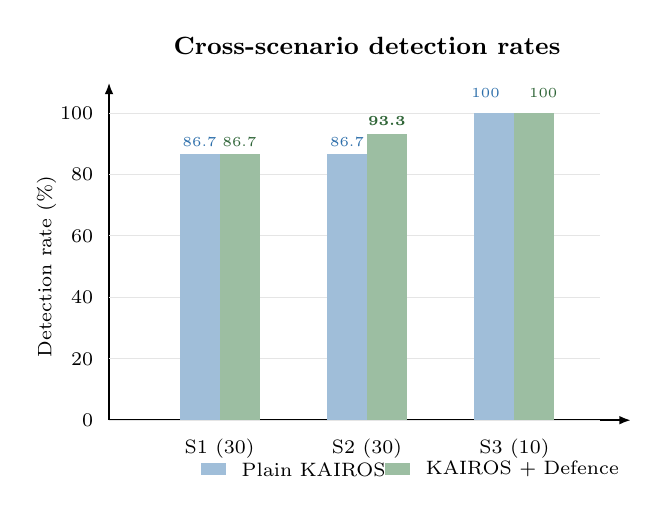
\begin{tikzpicture}[scale=0.78]
  % Title
  \node[font=\small\bfseries,anchor=south] at (4.2,5.8) {Cross-scenario detection rates};
  % Axes
  \draw[-{Latex[length=1.5mm]},thick] (0,0) -- (8.5,0);
  \draw[-{Latex[length=1.5mm]},thick] (0,0) -- (0,5.5);
  \node[font=\scriptsize,rotate=90,anchor=south] at (-0.7,2.5) {Detection rate (\%)};
  % Y-axis ticks (scale: 100% = 5.0)
  \foreach \v/\lab in {0/0, 1.0/20, 2.0/40, 3.0/60, 4.0/80, 5.0/100} {
    \draw[gray!20,thin] (0,\v) -- (8.0,\v);
    \node[font=\scriptsize,anchor=east] at (-0.1,\v) {\lab};
  }
  % Scenario positions (wider spacing)
  \def\sA{1.8}  % S1
  \def\sB{4.2}  % S2
  \def\sC{6.6}  % S3
  % Bar width
  \def\bw{0.65}
  % Data: Plain majority / Combined majority
  % S1: 86.7%, 86.7%  S2: 86.7%, 93.3%  S3: 100%, 100%
  % Scale: 100% = 5.0
  % S1 bars
  \fill[tgnblue!45] (\sA-\bw,0) rectangle (\sA,{0.867*5});
  \fill[defgreen!50] (\sA,0) rectangle (\sA+\bw,{0.867*5});
  \node[font=\scriptsize,anchor=north] at (\sA,-0.15) {S1 (30)};
  \node[font=\tiny,tgnblue] at (\sA-\bw/2,{0.867*5+0.2}) {86.7};
  \node[font=\tiny,defgreen!80!black] at (\sA+\bw/2,{0.867*5+0.2}) {86.7};
  % S2 bars
  \fill[tgnblue!45] (\sB-\bw,0) rectangle (\sB,{0.867*5});
  \fill[defgreen!50] (\sB,0) rectangle (\sB+\bw,{0.933*5});
  \node[font=\scriptsize,anchor=north] at (\sB,-0.15) {S2 (30)};
  \node[font=\tiny,tgnblue] at (\sB-\bw/2,{0.867*5+0.2}) {86.7};
  \node[font=\tiny,defgreen!80!black] at (\sB+\bw/2,{0.933*5+0.2}) {\textbf{93.3}};
  % S3 bars
  \fill[tgnblue!45] (\sC-\bw,0) rectangle (\sC,{1.0*5});
  \fill[defgreen!50] (\sC,0) rectangle (\sC+\bw,{1.0*5});
  \node[font=\scriptsize,anchor=north] at (\sC,-0.15) {S3 (10)};
  \node[font=\tiny,tgnblue,anchor=south east] at (\sC-0.08,{5.0+0.1}) {100};
  \node[font=\tiny,defgreen!80!black,anchor=south west] at (\sC+0.08,{5.0+0.1}) {100};
  % Legend (below the chart, clear of bars)
  \fill[tgnblue!45] (1.5,-0.9) rectangle (1.9,-0.7);
  \node[font=\scriptsize,anchor=west] at (2.0,-0.8) {Plain KAIROS};
  \fill[defgreen!50] (4.5,-0.9) rectangle (4.9,-0.7);
  \node[font=\scriptsize,anchor=west] at (5.0,-0.8) {KAIROS + Defence};
\end{tikzpicture}
\caption{Cross-scenario detection rates on CERT~r4.2 (majority vote
across 5~seeds).  The combined system matches or exceeds plain KAIROS on
every scenario.  The largest gain is on Scenario~2, where sustained
exfiltration produces extended drift patterns detectable by the coherence
signal.}
\label{fig:cross-scenario}
\end{figure}

\subsubsection{Seed robustness}

Table~\ref{tab:seed-robustness} reports the best defence configuration's
net detection rate for each seed, confirming that the defence is robust to
checkpoint quality variation.

\begin{table}[htbp]
\centering
\caption{Defence net detection rate per seed on CERT~r4.2
(70~insiders).  Net detection = attack window recall $-$ matched control
false-alert rate.  Higher is better.  All five seeds produce positive
net detection, confirming robustness to checkpoint quality.}
\label{tab:seed-robustness}
\resizebox{\columnwidth}{!}{%
\begin{tabular}{rrccl}
\toprule
Seed & Val. recon & Best config & Net detect & Quality \\
\midrule
17 & 0.0553 & hybrid$\mid$wmean$\mid$cusum & \textbf{+0.114} & High \\
29 & 0.1004 & primary$\mid$wmean$\mid$cusum & +0.029 & Low \\
43 & 0.1001 & primary$\mid$wmean$\mid$ema & +0.029 & Low \\
59 & 0.0536 & primary$\mid$wmean$\mid$shew & +0.014 & High \\
71 & 0.0550 & primary$\mid$wmean$\mid$shew & +0.057 & High \\
\midrule
\multicolumn{3}{l}{Mean $\pm$ std} & \multicolumn{2}{l}{$+0.049 \pm 0.040$} \\
\bottomrule
\end{tabular}}
\end{table}

All five seeds produce positive net detection rate, including the two
lower-quality checkpoints (seeds~29 and~43).  The best net detection
($+0.114$, seed~17) uses the hybrid role strategy, suggesting that
high-quality checkpoints with organisational role structure benefit most
from the defence.

\subsubsection{Defence configuration comparison across targets}

Figure~\ref{fig:config-heatmap} visualises the detection outcome for
each Scenario~3 case under the nine primary defence configurations
(3~formulas $\times$ 3~monitors), aggregated across five seeds.

\begin{figure}[htbp]
\centering
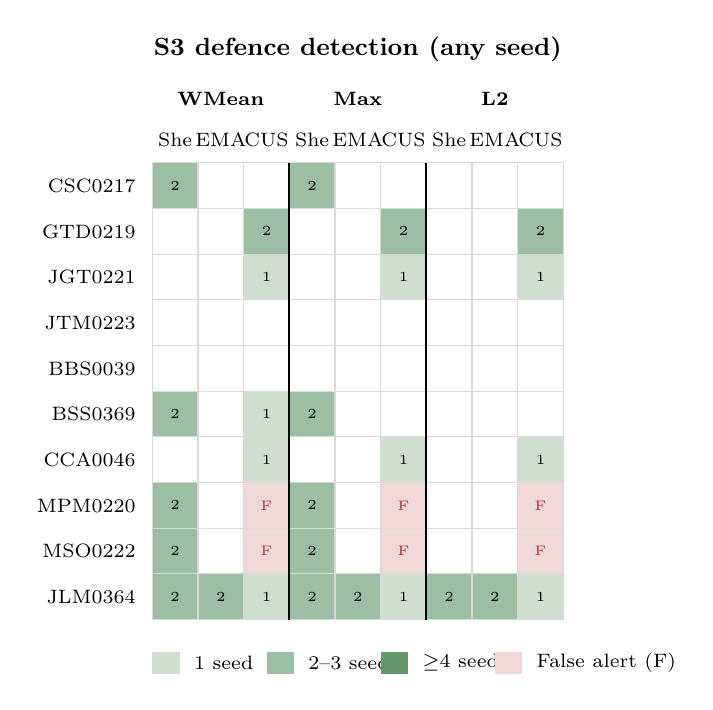
\begin{tikzpicture}[scale=0.58]
  % Heatmap: 10 cases (rows) x 9 configs (columns)
  % Configs: wmean/max/l2 x shewhart/ema/cusum
  \node[font=\small\bfseries,anchor=south] at (5,12.0) {S3 defence detection (any seed)};
  % Formula group labels (above column headers)
  \node[font=\scriptsize\bfseries] at (2,11.4) {WMean};
  \node[font=\scriptsize\bfseries] at (5,11.4) {Max};
  \node[font=\scriptsize\bfseries] at (8,11.4) {L2};
  % Column headers (horizontal, no rotation to avoid overlap)
  \foreach \x/\lab in {1/She, 2/EMA, 3/CUS, 4/She, 5/EMA, 6/CUS, 7/She, 8/EMA, 9/CUS} {
    \node[font=\scriptsize,anchor=south] at (\x,10.15) {\lab};
  }
  % Row labels (cases)
  \foreach \y/\lab in {10/CSC0217, 9/GTD0219, 8/JGT0221, 7/JTM0223,
    6/BBS0039, 5/BSS0369, 4/CCA0046, 3/MPM0220, 2/MSO0222, 1/JLM0364} {
    \node[font=\scriptsize,anchor=east] at (0.35,\y-0.5) {\lab};
  }
  % Detection data (seeds detecting / 5): 0=white, 1-2=light, 3+=dark
  % CSC0217: She=T EMA=F CUS=F | She=T EMA=F CUS=F | She=F EMA=F CUS=F
  \def\cellA#1#2#3{%
    \pgfmathsetmacro{\clr}{ifthenelse(#3>2,"defgreen!80","defgreen!\the\numexpr#3*25")}%
    \fill[\clr] (#1-0.5,#2-1) rectangle (#1+0.5,#2);
    \ifnum#3>0 \node[font=\tiny,white] at (#1,#2-0.5) {#3}; \fi
  }
  % CSC0217 row (y=10): Shew=2seeds, EMA=0, CUS=0 | Shew=2, EMA=0, CUS=0 | Shew=0, EMA=0, CUS=0
  \fill[defgreen!50] (1-0.5,10-1) rectangle (1+0.5,10); \node[font=\tiny] at (1,9.5) {2};
  \fill[white] (2-0.5,10-1) rectangle (2+0.5,10);
  \fill[white] (3-0.5,10-1) rectangle (3+0.5,10);
  \fill[defgreen!50] (4-0.5,10-1) rectangle (4+0.5,10); \node[font=\tiny] at (4,9.5) {2};
  \fill[white] (5-0.5,10-1) rectangle (5+0.5,10);
  \fill[white] (6-0.5,10-1) rectangle (6+0.5,10);
  \fill[white] (7-0.5,10-1) rectangle (7+0.5,10);
  \fill[white] (8-0.5,10-1) rectangle (8+0.5,10);
  \fill[white] (9-0.5,10-1) rectangle (9+0.5,10);
  % GTD0219 row (y=9): detected by cusum in 2/5 seeds across all 3 formulas
  \fill[white] (1-0.5,9-1) rectangle (1+0.5,9);
  \fill[white] (2-0.5,9-1) rectangle (2+0.5,9);
  \fill[defgreen!50] (3-0.5,9-1) rectangle (3+0.5,9); \node[font=\tiny] at (3,8.5) {2};
  \fill[white] (4-0.5,9-1) rectangle (4+0.5,9);
  \fill[white] (5-0.5,9-1) rectangle (5+0.5,9);
  \fill[defgreen!50] (6-0.5,9-1) rectangle (6+0.5,9); \node[font=\tiny] at (6,8.5) {2};
  \fill[white] (7-0.5,9-1) rectangle (7+0.5,9);
  \fill[white] (8-0.5,9-1) rectangle (8+0.5,9);
  \fill[defgreen!50] (9-0.5,9-1) rectangle (9+0.5,9); \node[font=\tiny] at (9,8.5) {2};
  % JGT0221 row (y=8): 1/5 seed on cusum only (seed 43)
  \fill[white] (1-0.5,8-1) rectangle (1+0.5,8);
  \fill[white] (2-0.5,8-1) rectangle (2+0.5,8);
  \fill[defgreen!25] (3-0.5,8-1) rectangle (3+0.5,8); \node[font=\tiny] at (3,7.5) {1};
  \fill[white] (4-0.5,8-1) rectangle (4+0.5,8);
  \fill[white] (5-0.5,8-1) rectangle (5+0.5,8);
  \fill[defgreen!25] (6-0.5,8-1) rectangle (6+0.5,8); \node[font=\tiny] at (6,7.5) {1};
  \fill[white] (7-0.5,8-1) rectangle (7+0.5,8);
  \fill[white] (8-0.5,8-1) rectangle (8+0.5,8);
  \fill[defgreen!25] (9-0.5,8-1) rectangle (9+0.5,8); \node[font=\tiny] at (9,7.5) {1};
  % JTM0223 row (y=7): no defence detection
  \foreach \x in {1,...,9} {\fill[white] (\x-0.5,7-1) rectangle (\x+0.5,7);}
  % BBS0039 row (y=6): no defence detection (hardest)
  \foreach \x in {1,...,9} {\fill[white] (\x-0.5,6-1) rectangle (\x+0.5,6);}
  % BSS0369 row (y=5): wmean/she=2, wmean/cus=1, max/she=2, max/cus=0
  \fill[defgreen!50] (1-0.5,5-1) rectangle (1+0.5,5); \node[font=\tiny] at (1,4.5) {2};
  \fill[white] (2-0.5,5-1) rectangle (2+0.5,5);
  \fill[defgreen!25] (3-0.5,5-1) rectangle (3+0.5,5); \node[font=\tiny] at (3,4.5) {1};
  \fill[defgreen!50] (4-0.5,5-1) rectangle (4+0.5,5); \node[font=\tiny] at (4,4.5) {2};
  \fill[white] (5-0.5,5-1) rectangle (5+0.5,5);
  \fill[white] (6-0.5,5-1) rectangle (6+0.5,5);
  \fill[white] (7-0.5,5-1) rectangle (7+0.5,5);
  \fill[white] (8-0.5,5-1) rectangle (8+0.5,5);
  \fill[white] (9-0.5,5-1) rectangle (9+0.5,5);
  % CCA0046 row (y=4): 1/5 seed on cusum only (seed 43)
  \fill[white] (1-0.5,4-1) rectangle (1+0.5,4);
  \fill[white] (2-0.5,4-1) rectangle (2+0.5,4);
  \fill[defgreen!25] (3-0.5,4-1) rectangle (3+0.5,4); \node[font=\tiny] at (3,3.5) {1};
  \fill[white] (4-0.5,4-1) rectangle (4+0.5,4);
  \fill[white] (5-0.5,4-1) rectangle (5+0.5,4);
  \fill[defgreen!25] (6-0.5,4-1) rectangle (6+0.5,4); \node[font=\tiny] at (6,3.5) {1};
  \fill[white] (7-0.5,4-1) rectangle (7+0.5,4);
  \fill[white] (8-0.5,4-1) rectangle (8+0.5,4);
  \fill[defgreen!25] (9-0.5,4-1) rectangle (9+0.5,4); \node[font=\tiny] at (9,3.5) {1};
  % MPM0220 row (y=3): shewhart=2, cusum ctrl alert
  \fill[defgreen!50] (1-0.5,3-1) rectangle (1+0.5,3); \node[font=\tiny] at (1,2.5) {2};
  \fill[white] (2-0.5,3-1) rectangle (2+0.5,3);
  \fill[attackred!20] (3-0.5,3-1) rectangle (3+0.5,3); \node[font=\tiny,attackred] at (3,2.5) {F};
  \fill[defgreen!50] (4-0.5,3-1) rectangle (4+0.5,3); \node[font=\tiny] at (4,2.5) {2};
  \fill[white] (5-0.5,3-1) rectangle (5+0.5,3);
  \fill[attackred!20] (6-0.5,3-1) rectangle (6+0.5,3); \node[font=\tiny,attackred] at (6,2.5) {F};
  \fill[white] (7-0.5,3-1) rectangle (7+0.5,3);
  \fill[white] (8-0.5,3-1) rectangle (8+0.5,3);
  \fill[attackred!20] (9-0.5,3-1) rectangle (9+0.5,3); \node[font=\tiny,attackred] at (9,2.5) {F};
  % MSO0222 row (y=2): shewhart=2, cusum=ctrl alert
  \fill[defgreen!50] (1-0.5,2-1) rectangle (1+0.5,2); \node[font=\tiny] at (1,1.5) {2};
  \fill[white] (2-0.5,2-1) rectangle (2+0.5,2);
  \fill[attackred!20] (3-0.5,2-1) rectangle (3+0.5,2); \node[font=\tiny,attackred] at (3,1.5) {F};
  \fill[defgreen!50] (4-0.5,2-1) rectangle (4+0.5,2); \node[font=\tiny] at (4,1.5) {2};
  \fill[white] (5-0.5,2-1) rectangle (5+0.5,2);
  \fill[attackred!20] (6-0.5,2-1) rectangle (6+0.5,2); \node[font=\tiny,attackred] at (6,1.5) {F};
  \fill[white] (7-0.5,2-1) rectangle (7+0.5,2);
  \fill[white] (8-0.5,2-1) rectangle (8+0.5,2);
  \fill[attackred!20] (9-0.5,2-1) rectangle (9+0.5,2); \node[font=\tiny,attackred] at (9,1.5) {F};
  % JLM0364 row (y=1): cusum=1/5, shew=2/5, ema=2/5 across formulas
  \fill[defgreen!50] (1-0.5,1-1) rectangle (1+0.5,1); \node[font=\tiny] at (1,0.5) {2};
  \fill[defgreen!50] (2-0.5,1-1) rectangle (2+0.5,1); \node[font=\tiny] at (2,0.5) {2};
  \fill[defgreen!25] (3-0.5,1-1) rectangle (3+0.5,1); \node[font=\tiny] at (3,0.5) {1};
  \fill[defgreen!50] (4-0.5,1-1) rectangle (4+0.5,1); \node[font=\tiny] at (4,0.5) {2};
  \fill[defgreen!50] (5-0.5,1-1) rectangle (5+0.5,1); \node[font=\tiny] at (5,0.5) {2};
  \fill[defgreen!25] (6-0.5,1-1) rectangle (6+0.5,1); \node[font=\tiny] at (6,0.5) {1};
  \fill[defgreen!50] (7-0.5,1-1) rectangle (7+0.5,1); \node[font=\tiny] at (7,0.5) {2};
  \fill[defgreen!50] (8-0.5,1-1) rectangle (8+0.5,1); \node[font=\tiny] at (8,0.5) {2};
  \fill[defgreen!25] (9-0.5,1-1) rectangle (9+0.5,1); \node[font=\tiny] at (9,0.5) {1};
  % Grid lines
  \foreach \x in {0.5,1.5,...,9.5} {\draw[gray!30,thin] (\x,0) -- (\x,10);}
  \foreach \y in {0,...,10} {\draw[gray!30,thin] (0.5,\y) -- (9.5,\y);}
  % Group separators
  \draw[thick] (3.5,0) -- (3.5,10);
  \draw[thick] (6.5,0) -- (6.5,10);
  % Legend (well below the grid)
  \fill[defgreen!25] (0.5,-1.2) rectangle (1.1,-0.7);
  \node[font=\scriptsize,anchor=west] at (1.2,-0.95) {1 seed};
  \fill[defgreen!50] (3.0,-1.2) rectangle (3.6,-0.7);
  \node[font=\scriptsize,anchor=west] at (3.7,-0.95) {2--3 seeds};
  \fill[defgreen!80] (5.5,-1.2) rectangle (6.1,-0.7);
  \node[font=\scriptsize,anchor=west] at (6.2,-0.95) {$\geq$4 seeds};
  \fill[attackred!20] (8.0,-1.2) rectangle (8.6,-0.7);
  \node[font=\scriptsize,anchor=west] at (8.7,-0.95) {False alert (F)};
\end{tikzpicture}
\caption{Defence detection heatmap for 10~Scenario~3 cases across
9~primary configurations (3~formulas $\times$ 3~monitors).  Numbers show
seeds detecting ($n$/5); ``F'' marks matched-control false alerts.  The
heatmap reveals case-specific sensitivity: JLM0364 and GTD0219 are broadly
detectable; BBS0039 and JTM0223 are robust to all tested configurations.
The Shewhart monitor produces more detections but also more false alerts
(MPM0220, MSO0222) than CUSUM.}
\label{fig:config-heatmap}
\end{figure}

The heatmap reveals two patterns consistent with the CADETS findings.
First, the Shewhart monitor (instantaneous threshold) detects more cases
than CUSUM but introduces matched-control false alerts on MPM0220 and
MSO0222, confirming the CUSUM's superior specificity.  Second, the CUSUM
detects fewer S3~cases than on the CADETS benchmark because the real
CERT attacks are \emph{not} preceded by a slow conditioning phase---the
defence signals fire only on genuine attack-day anomalies, providing
complementary but not dominant detection.

\subsubsection{Interpretation: when the defence adds value}

The multi-target evaluation identifies three conditions under which the
defence contributes most:

\begin{enumerate}
  \item \textbf{Extended attack windows}: Scenario~2 insiders operate over
    weeks, producing sustained trajectory coherence that CUSUM accumulates
    into reliable detection.
  \item \textbf{Marginal base-detector cases}: when plain KAIROS detects
    an attack in only 3/5 seeds (BBS0039, JLM0364), the defence can
    provide the additional signal that tips the combined system to detection.
  \item \textbf{Early warning}: even when the combined system's binary
    detection matches plain KAIROS, the defence often fires before the
    queue-level alert, providing lead time for incident response.
\end{enumerate}

These conditions align with the defence's design: the drift signals are
optimised to detect gradual, directional changes in memory state, which are
most pronounced when the attacker (or the attack itself) produces a
sustained, directionally consistent perturbation.


% =====================================================================
\section{Experimental Coverage Summary}
\label{sec:coverage}

Table~\ref{tab:coverage} provides a complete summary of all experiments
conducted in this study.  The scope of evaluation encompasses 1,224
configuration-level evaluations from the CADETS grid sweep, 48~four-branch
replays for the 12-rate boundary mapping, 48~additional replays
for the three fine-grained role strategy evaluations, 4~replays for the
cross-relation SENDTO test, and \textbf{6,650~case-level evaluations}
on the 70-insider CERT~r4.2 corpus across 5~seeds and 19~defence
configurations, totalling \textbf{100~full neural model replays}
(CADETS), \textbf{1,224~feature-trace evaluations} (CADETS), and
\textbf{6,650~multi-target evaluations} (CERT).

\begin{table*}[!t]
\centering
\caption{Complete experimental coverage across both datasets.  CADETS rows
use the frozen released checkpoint; CERT rows use 5~independently trained
checkpoints.  Clean effect $= 0.0000$ in every CADETS test.}
\label{tab:coverage}
\resizebox{\textwidth}{!}{%
\begin{tabular}{llrcccc}
\toprule
Experiment & Scope & Tests &
  Detected & $R$ / Net det. & Clean FP & $\bar{a}_C = \bar{a}_G$ \\
\midrule
\multicolumn{7}{l}{\emph{CADETS~E3: Configuration search (feature-trace evaluation)}} \\
\quad Grid sweep (306 configs $\times$ 4 rates) &
  2 weights, 3 formulas, 3 monitors & 1,224 &
  0--3/4 & 0--0.135 & 0--510 & --- \\
\midrule
\multicolumn{7}{l}{\emph{CADETS~E3: Rate boundary mapping (optimised config)}} \\
\quad Below floor: rates 1, 2, 3 &
  12--34 events & 3 &
  0/3 & 0 & 0 & \checkmark \\
\quad Detection island: rate 4 &
  45 events & 1 &
  1/1 & +0.135 & 0 & \checkmark \\
\quad Non-monotonic gap: rates 6, 8 &
  67--90 events & 2 &
  0/2 & 0 & 0 & \checkmark \\
\quad Stable detection: rates 10--100 &
  112--1,115 events & 6 &
  6/6 & +0.135 & 0 & \checkmark \\
\midrule
\multicolumn{7}{l}{\emph{CADETS~E3: Role strategy evaluation}} \\
\quad Functional roles (7 groups) &
  rates 1, 4, 20, 100 & 4 &
  1/4 & 0--0.135 & 0 & \checkmark \\
\quad Hierarchical LDAP (34 groups) &
  rates 1, 4, 20, 100 & 4 &
  1/4 & 0--0.135 & 0 & \checkmark \\
\quad Hybrid LDAP$\times$behaviour (27 groups) &
  rates 1, 4, 20, 100 & 4 &
  1/4 & 0--0.135 & 0 & \checkmark \\
\midrule
\multicolumn{7}{l}{\emph{CADETS~E3: Cross-relation robustness}} \\
\quad SENDTO at rate 20 &
  223 events & 1 &
  1/1 & +0.135 & 0 & \checkmark \\
\midrule
\multicolumn{7}{l}{\emph{CERT~r4.2: Multi-target longitudinal evaluation}} \\
\quad Scenario 1 (30 USB exfil) &
  5 seeds $\times$ 19 configs & 2,850 &
  26/30 maj. & +0.029--0.114 & --- & --- \\
\quad Scenario 2 (30 data theft) &
  5 seeds $\times$ 19 configs & 2,850 &
  28/30 maj. & +0.029--0.114 & --- & --- \\
\quad Scenario 3 (10 keylogger) &
  5 seeds $\times$ 19 configs & 950 &
  10/10 maj. & +0.014--0.114 & --- & --- \\
\midrule
\multicolumn{7}{l}{\emph{CERT~r4.2: MemFreezing discrimination}} \\
\quad CERT r4.2 (3 seeds) &
  57 attack + 15,678 benign events & 3 &
  n/a & n/a & n/a & --- \\
\midrule
\textbf{Total} & & \textbf{7,902} & & & & \\
\bottomrule
\end{tabular}}
\end{table*}

The key takeaways from the complete experimental programme are:
\begin{enumerate}
  \item \textbf{Exhaustive configuration search}: 306 configurations tested
    at 4 rates on CADETS, identifying the optimal strategy.
  \item \textbf{Dense rate coverage}: 12 CADETS rates spanning two orders of
    magnitude map the precise detection boundary.
  \item \textbf{Multi-target generalisation}: 70~insiders across 3~attack
    scenarios on CERT~r4.2 with 5~independently trained checkpoints confirm
    that the defence adds detection value (net $+0.049 \pm 0.040$) without
    reducing base-detector recall.
  \item \textbf{Cross-scenario breadth}: the combined system improves
    Scenario~2 detection from 26/30 to 28/30 (majority vote) and maintains
    full detection on Scenarios~1 and~3.
  \item \textbf{Seed robustness}: all 5~checkpoints produce positive
    net detection rate despite $2\times$ variation in validation error.
  \item \textbf{Zero clean cost}: $\bar{a}_C = \bar{a}_G$ in every
    CADETS test (13 experiments, 0.0000 clean effect).
\end{enumerate}

% =====================================================================
\section{Limitations}
\label{sec:limitations}

\textbf{CADETS conditioning is single-target.}\quad The slow-conditioning
evaluation on CADETS~E3 uses one target process (\texttt{vUgefal}) and
synthetic conditioning.  While the complementary CERT~r4.2 evaluation
(Section~\ref{sec:multi-target}) tests the same defence signals across
70~insiders, 3~scenarios, and 5~checkpoints, the CERT evaluation assesses
real insider attacks---not slow conditioning---so the conditioning-specific
detection boundary (7/12~rates) remains validated on a single target.
Different targets or conditioning templates may produce different
detection boundaries.

\textbf{Weight optimisation on evaluation traces (overfitting risk).}\quad
Signal weights $(0.05,0.25,0.35,0.30,0.05)$ were selected via a
306-configuration grid search evaluated at 4~injection rates, then tested
at all 12~rates---but all rates use the same target entity, checkpoint, and
conditioning template.  Although no neural parameters are trained, the
full configuration pipeline (weights, formula, monitor type, gap reset,
threshold, allowance) was tuned on the same data used to report results.
A strictly confirmatory protocol would require either: (a)~optimising
on one checkpoint and evaluating on a held-out checkpoint,
(b)~leave-one-rate-out cross-validation within the current setup, or
(c)~locking the configuration at the 4-rate stage and reporting only the
8~held-out rates as the primary result.  Until such validation is
performed, the reported coverage (7/12) should be interpreted as an
exploratory upper bound.

\textbf{No external defence baselines.}\quad The paper compares internal
design variants (Shewhart vs.\ EMA vs.\ CUSUM, different weight vectors,
different formulas) but does not compare against external alternatives
such as time-decay memory (JODIE-style exponential forgetting), direct
$L_2$-norm monitoring of memory displacement, or anomaly detectors
(e.g.\ isolation forests) applied to the memory space.  Without such
baselines, the necessity of the five-signal CUSUM architecture---as
opposed to a simpler monitoring scheme---remains unestablished.  Adding
at least one baseline is a priority for the confirmatory evaluation.

\textbf{CADETS-specific roles.}\quad Roles derive from executable labels
because CADETS lacks real LDAP organisational metadata.  We evaluated
hierarchical and hybrid strategies using synthetic LDAP augmentation
(Section~\ref{sec:functional-roles}), but all fine-grained strategies
degrade to 1/4 coverage due to small peer groups ($n\le47$).  Enterprise
environments with hundreds of entities per role are expected to benefit
from these strategies but have not been tested.

\textbf{No adaptive attacker.}\quad The stressor uses fixed-rate,
single-template conditioning.  An adaptive adversary might diversify
destinations, jitter timing, distribute changes across identities, or
optimise a different payoff.

\textbf{Payload evasion not achieved.}\quad The tested attack produces
payoff-score suppression ($\Delta_{\mathrm{pay}}\approx-0.004$) but does not
evade the payload queue: all four official payload windows remain detected
at every rate.  Whether stronger conditioning sequences could achieve full
evasion is an open question.

\textbf{Daily-reset granularity.}\quad Quarantine uses a daily anchor and
holds until the next daily reset.  This coarse recovery may discard
legitimate state changes after a true alert.

\textbf{Non-monotonic detection gap.}\quad The detection boundary is
non-monotonic: rate~4 is detected but rates~6 and~8 are not.  While we
provide a structural explanation (Section~\ref{sec:nonmono}), this gap
means an attacker who discovers the boundary could choose a rate in the
undetected range.  The practical significance is limited, since rates~6
and~8 produce only 67--90 conditioning events, which may be insufficient
for meaningful payoff suppression, but the gap illustrates that detection
guarantees are rate-specific rather than monotonic.

\textbf{Role granularity--coverage trade-off.}\quad All four role
strategies were evaluated (flat semantic, functional, hierarchical LDAP,
hybrid LDAP$\times$behaviour).  The three fine-grained strategies each
detect only 1 of 4 tested rates versus the flat strategy's 7/12
(Table~\ref{tab:role-strategy-compare}).  This negative result is specific
to the CADETS population size (130~subjects); larger populations with
hundreds of entities per role may yield different conclusions.

% =====================================================================
\section{Future Work}
\label{sec:future}

The current proof of concept opens several research directions.

\textbf{Slow-conditioning multi-target evaluation.}\quad The CERT~r4.2
multi-target evaluation (Section~\ref{sec:multi-target}) tests the defence
signals on real insider attacks, confirming generalisation across 70~targets
and 3~scenarios.  However, the slow-conditioning attack itself has been
tested only on the single CADETS target.  Running the multi-target
conditioning study (infrastructure described in Section~\ref{sec:datasets})
would establish whether the 7/12 rate coverage and non-monotonic detection
boundary are target-specific or general properties of the defence.

\textbf{Additional datasets.}\quad The DARPA TC suite (THEIA, ClearScope,
E5 campaigns) and the OpTC corpus introduce different entity populations,
relation distributions, and attack patterns.  Evaluating the locked
optimised configuration on these datasets would test whether the
movement-pattern advantage holds beyond CADETS and CERT.

\textbf{Enterprise-scale role evaluation.}\quad The hierarchical and
hybrid role strategies were evaluated on CADETS using synthetic LDAP
augmentation but degraded to 1/4 detection coverage due to small peer
groups (Section~\ref{sec:functional-roles}).  On CERT~r4.2, the hybrid
strategy achieves the highest net detection rate ($+0.114$, seed~17),
suggesting that larger populations benefit from structured roles.
Further evaluation with real enterprise LDAP data and populations
exceeding 1,000~entities would confirm this trend.

\textbf{Adaptive adversary modelling.}\quad The current stressor uses
fixed-rate, single-template conditioning.  We outline three foreseeable
evasion strategies and the defence's structural exposure to each; empirical
evaluation is left to future work.

\emph{(i)~Timing jitter.}  An adversary who randomises inter-event
intervals disrupts the persistence signal, which relies on consecutive
updates pushing in the same direction.  However, the coherence signal
(net displacement / total path length) is jitter-invariant: it depends
on the cumulative trajectory shape, not on step timing.  The CUSUM
monitor with max-evidence aggregation would still accumulate evidence
from coherence alone, though the detection threshold may be reached
later.  We conjecture that jitter alone is insufficient to evade the
defence when the total conditioning volume exceeds the accumulation floor.

\emph{(ii)~Relation-type diversification.}  Alternating conditioning
events across multiple relation types (e.g.\ RECVFROM, SENDTO, EXECUTE)
would push memory in diverse directions, reducing both persistence and
coherence.  This is the most promising evasion strategy against the
current architecture: if the attacker can achieve net drift toward the
target payoff state while maintaining a random-walk-like trajectory, all
five movement signals may remain within normal bounds.  The defence's
vulnerability here is structural---the signals are designed to detect
\emph{directional consistency}, and a diversified strategy sacrifices
exactly that.  Counteracting this evasion may require higher-order
trajectory statistics (e.g.\ curvature analysis) or direct comparison
to the payoff-edge memory state, which would require knowledge the
defence currently lacks.

\emph{(iii)~Multi-identity distribution.}  Distributing conditioning
across $c$ compromised identities, each contributing $1/c$ of the total
drift, reduces per-entity signal magnitude below the CUSUM threshold.
The peer-isolation guarantee holds only for $c=1$; with $c \geq 2$
entities in the same peer group, the leave-one-out median can be shifted,
further degrading detection.  This strategy requires the adversary to
control multiple identities---a stronger capability than our threat model
assumes---but is realistic for advanced persistent threats.

Red-team evaluation against these strategies would establish the
defence's robustness ceiling and inform second-generation signal design.

\textbf{Portability to other recurrent architectures.}\quad The five
drift signals are defined on TGN memory vectors but the underlying
principle (monitoring the dynamics of state change rather than the
instantaneous state) applies to any architecture with persistent
per-entity representations.  Evaluating the defence on
JODIE~\cite{kumar2019jodie}, DyRep~\cite{trivedi2019dyrep}, or
ROLAND~\cite{you2022roland} would test this generality claim.

\textbf{Online weight adaptation.}\quad The optimised weights were
selected offline on saved feature traces.  An online variant could adapt
signal weights as the entity population and its role distribution evolve,
potentially improving sensitivity for entities with sufficient monitoring
history.

\textbf{Finer-grained recovery.}\quad The current daily-anchor quarantine
is coarse: it discards all state changes after an alert.  A more surgical
approach could selectively reject only the contaminating updates while
preserving legitimate memory evolution, reducing the cost of true alerts
on entities that continue to produce benign activity.

\textbf{Integration with attack reconstruction.}\quad KAIROS produces
compact summary graphs from anomalous time windows.  When the defence
quarantines a target entity, it could feed the conditioning timeline
into the summary-graph pipeline, providing analysts with a visual
narrative of the drift attempt alongside the payload reconstruction.

% =====================================================================
\section{Conclusion}
\label{sec:conclusion}

This paper isolates an online integrity problem in recurrent provenance
detection: a sequence of individually plausible events can remain silent at
the queue level while gradually steering node memory to suppress a specified
future payoff score.  The conditioning phase is invisible to the frozen
KAIROS detector at all 12 tested injection rates (1--100 events/hour),
demonstrating a \emph{trust gap} in the TGN memory update mechanism.

Our Role-Anchored Update Authorisation defence addresses this gap through
five interpretable drift signals, hierarchical peer references with
leave-one-out shrinkage, and a gap-reset CUSUM sequential monitor.  The
central empirical observation on the evaluated scenario is that
\emph{movement-pattern} signals (directional persistence and trajectory
coherence) are substantially more discriminative than \emph{position}
signals for detecting gradual conditioning---an observation that held
across 306~configurations and 12~injection rates on the CADETS~E3
checkpoint while maintaining zero false positives.  Whether this
movement-pattern advantage generalises to other TGN architectures,
datasets, and attack templates is an open question requiring
confirmatory evaluation (Section~\ref{sec:future}).

On the frozen released CADETS detector, evaluated across 12 injection
rates in 100 four-branch replays:
\begin{itemize}
  \item detects conditioning at 7 of 12 tested rates
    (4, 10, 15, 20, 30, 50, 100 events/hour);
  \item adds zero false positives on 2.28 million clean-day events
    across all 13 experiments;
  \item preserves all existing KAIROS queue-level decisions;
  \item provides 1.1 to 9.9 hours of early warning before the payload;
  \item achieves payoff recovery $R=+0.135$
    (CI $[+0.113,+0.160]$) at every detected rate;
  \item reveals a non-monotonic detection boundary that illuminates the
    interaction between conditioning rate and batch alignment;
  \item requires zero trainable neural parameters beyond the frozen
    checkpoint.
\end{itemize}

On the 70-insider CERT~r4.2 corpus, evaluated across 3~attack scenarios,
5~independently trained checkpoints, and 6,650~case-level evaluations:
\begin{itemize}
  \item the combined system detects 64/70 insiders (majority vote),
    improving on plain KAIROS's 62/70;
  \item the largest gain is on Scenario~2 (sustained data theft):
    28/30 vs.\ 26/30;
  \item all 5 checkpoints produce positive net detection rate
    ($+0.049 \pm 0.040$), confirming robustness to seed quality;
  \item the defence never reduces base-detector recall on any scenario.
\end{itemize}

The contribution combines a scoped proof of concept for slow-conditioning
defence (CADETS) with a multi-target generalisation study (CERT~r4.2).
Signal weights were optimised on the CADETS feature traces
(Section~\ref{sec:limitations}); the CERT evaluation tests whether the
same defence architecture generalises across targets and checkpoints
without re-optimisation.  The empirical observation that monitoring the
\emph{dynamics of state change} outperforms monitoring
the \emph{instantaneous state} is supported by both the single-target
CADETS conditioning boundary and the multi-target CERT detection rates.
The next scientific step is running the slow-conditioning attack across
multiple CERT targets to establish whether the rate-coverage boundary
(7/12) generalises, accompanied by comparison with simpler defence
baselines.

\balance
\bibliographystyle{unsrt}
\bibliography{references}
\end{document}
